\setcounter{section}{6}
\addsec{Versuch 6}

\subsection{Differenzverstärker (nur Simulation)}
\begin{figure}[H]
	\centering
	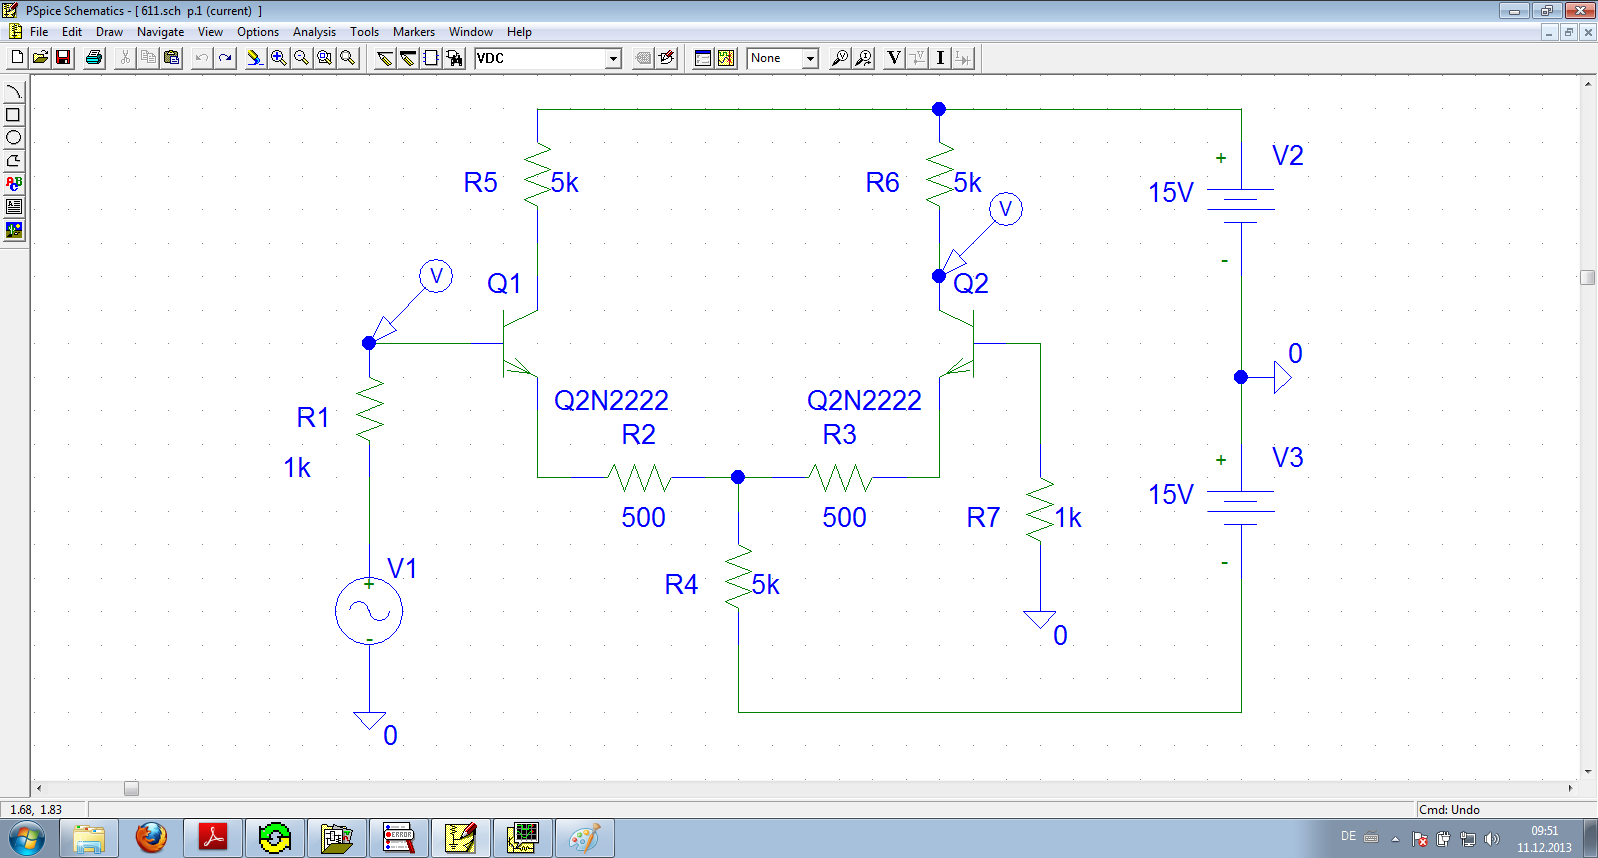
\includegraphics[width=\linewidth]{versuch6/spice/schem611.png}
	\caption{Schaltplan, wie im Skript vorgegeben}
\end{figure}
\begin{figure}[H]
	\centering
	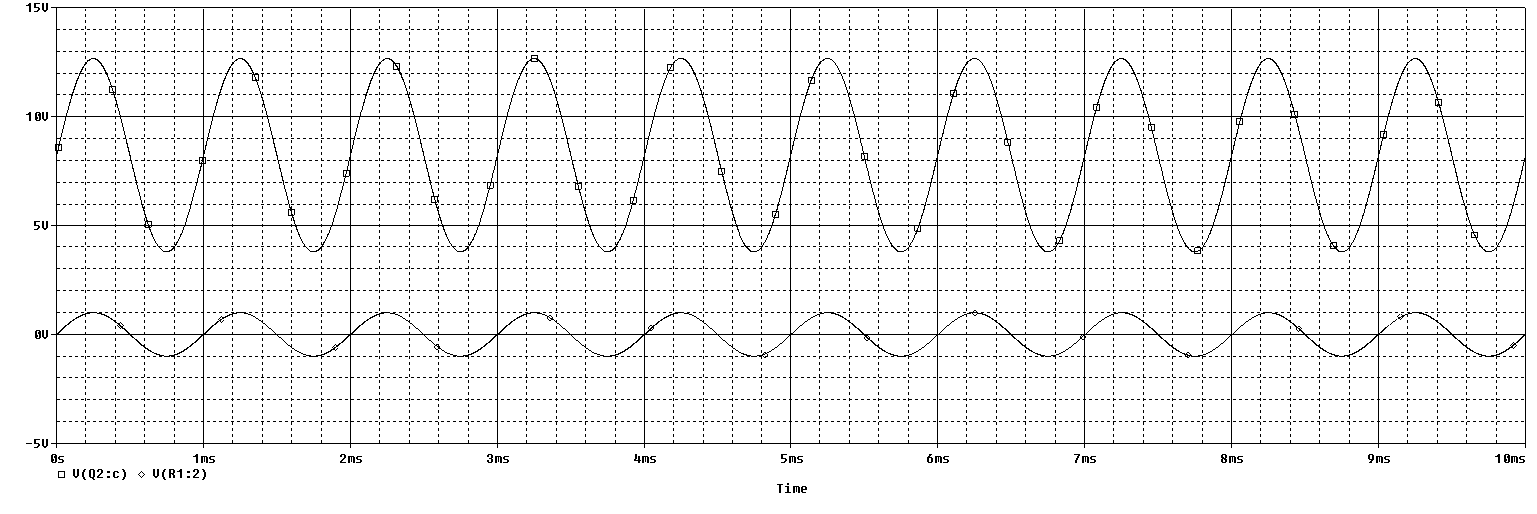
\includegraphics[width=\linewidth]{versuch6/spice/611.png}
	\caption{Simulationsergebnis}
\end{figure}
Die Gegentaktverstärkung der Schaltung wurde auf 4.2 bestimmt.
Dann wurde die Schaltung so geändert, dass die Signalquelle den invertierenden Eingang des Verstärkes treibt:
\begin{figure}[H]
	\centering
	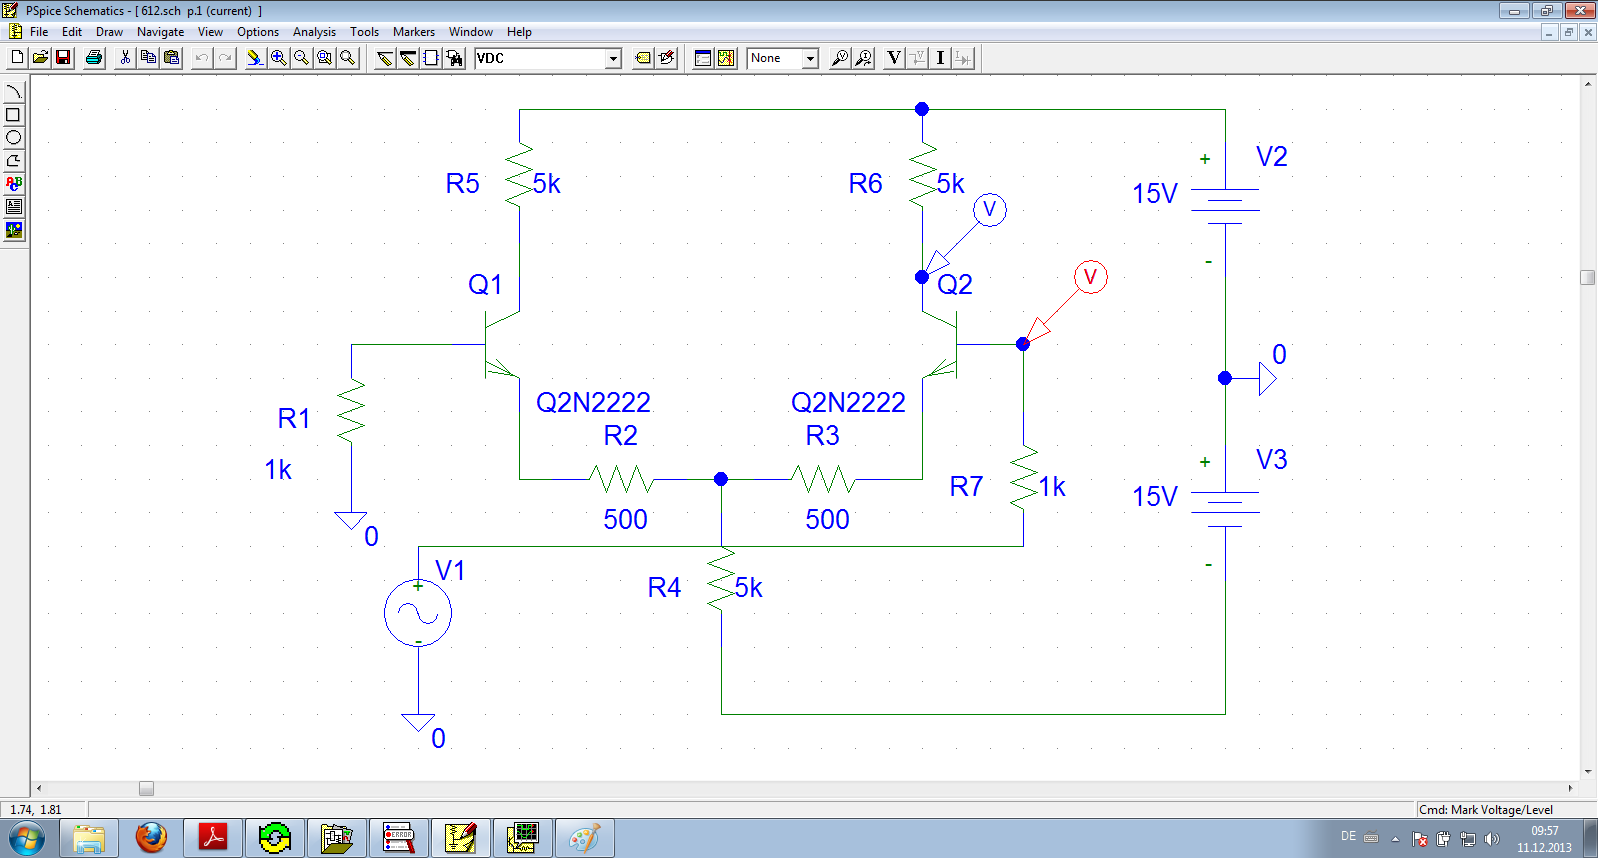
\includegraphics[width=\linewidth]{versuch6/spice/schem612.png}
	\caption{Schaltplan, wie im Skript vorgegeben}
\end{figure}
\begin{figure}[H]
	\centering
	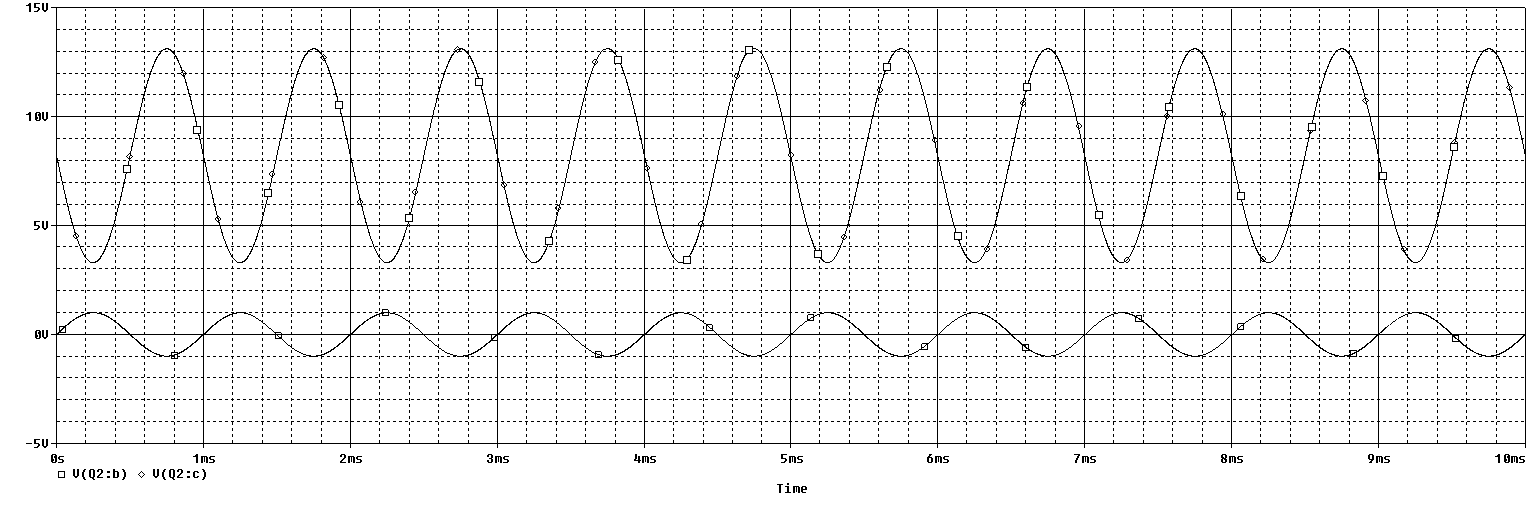
\includegraphics[width=\linewidth]{versuch6/spice/612.png}
	\caption{Simulationsergebnis}
\end{figure}
Die Gegentaktverstärkung der Schaltung wurde auf 4.8 bestimmt.
Dann wurde die Schaltung so geändert, dass beide Eingänge das selbe Signal bekommen:
\begin{figure}[H]
	\centering
	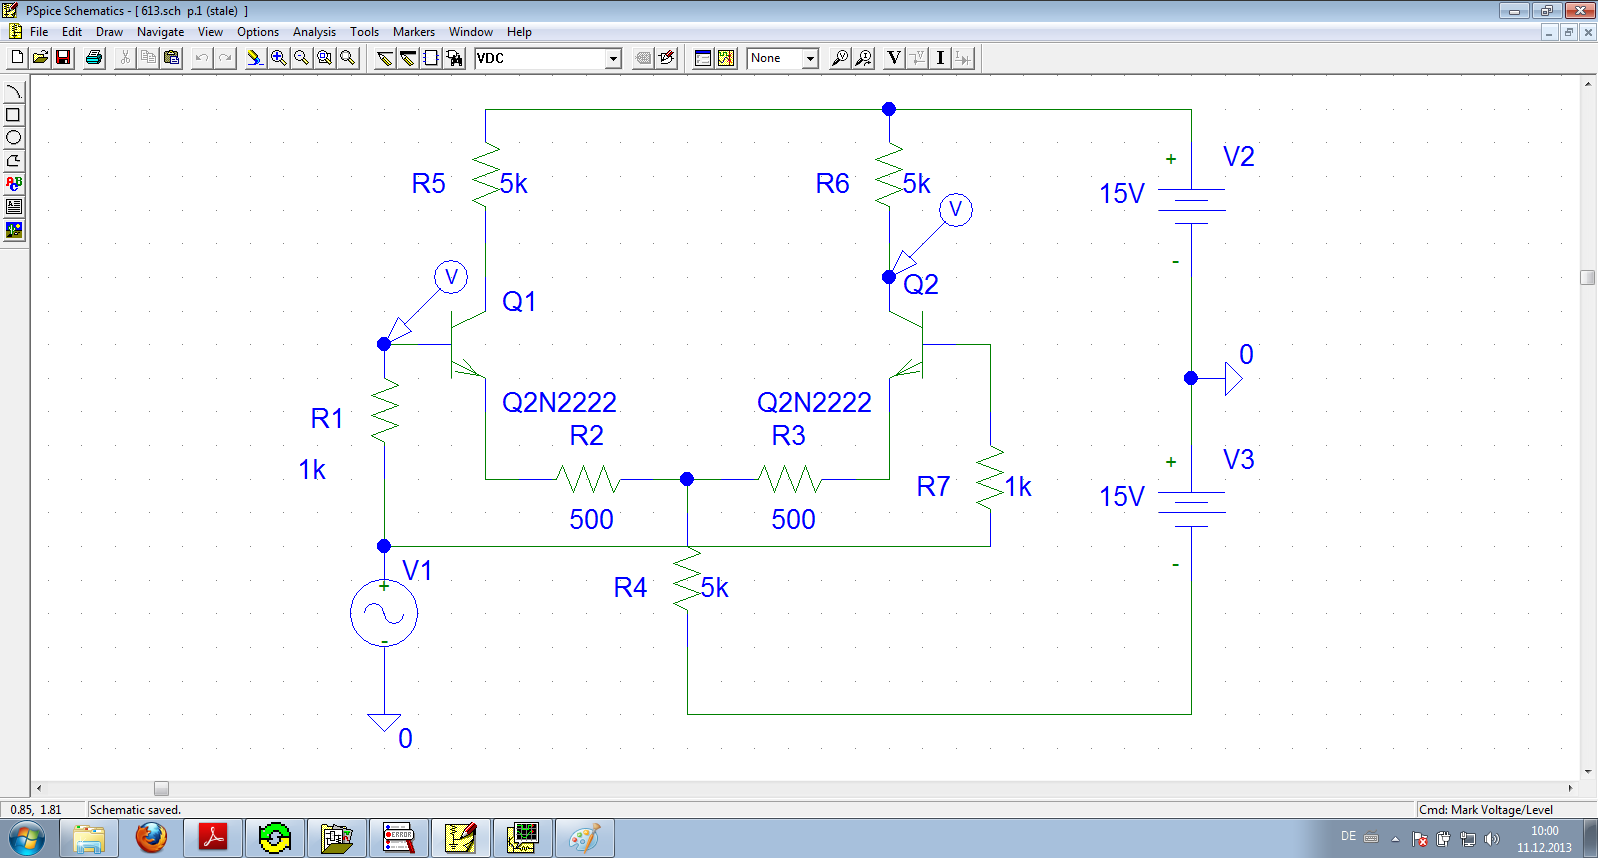
\includegraphics[width=\linewidth]{versuch6/spice/schem613.png}
	\caption{Schaltplan, wie im Skript vorgegeben}
\end{figure}
\begin{figure}[H]
	\centering
	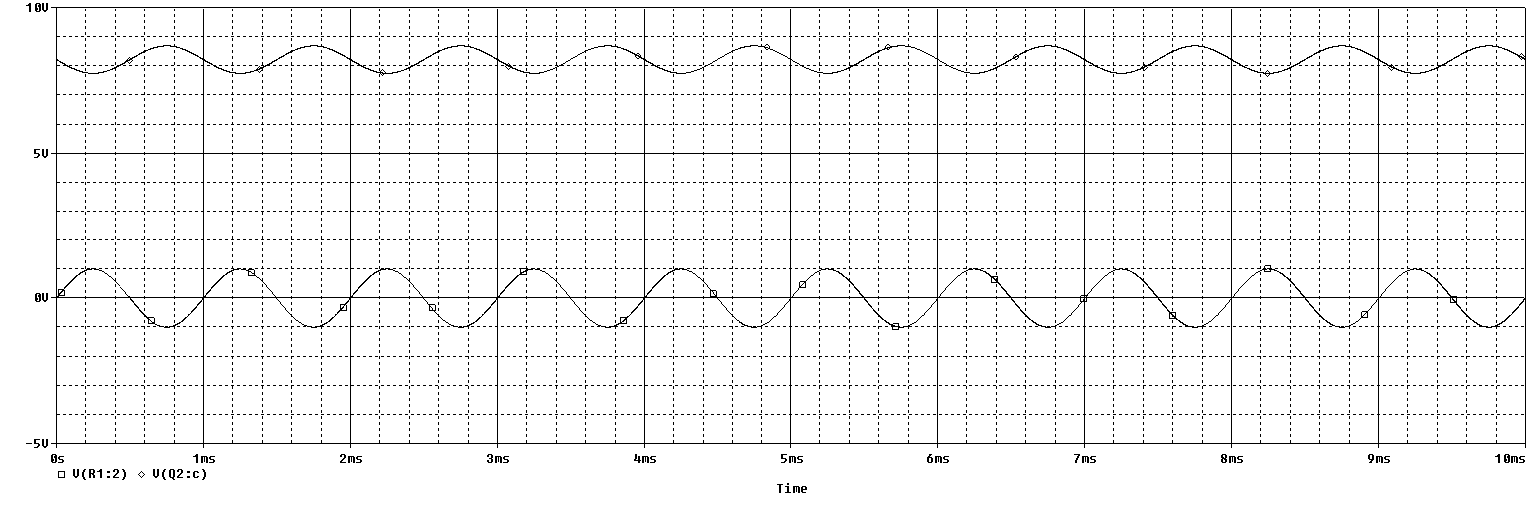
\includegraphics[width=\linewidth]{versuch6/spice/613.png}
	\caption{Simulationsergebnis}
\end{figure}
Die Gleichtaktverstärkung der Schaltung wurde auf 0.5 bestimmt.
Dann wurde $R_E$ durch eine Konstantstromquelle ersetzt
\begin{figure}[H]
	\centering
	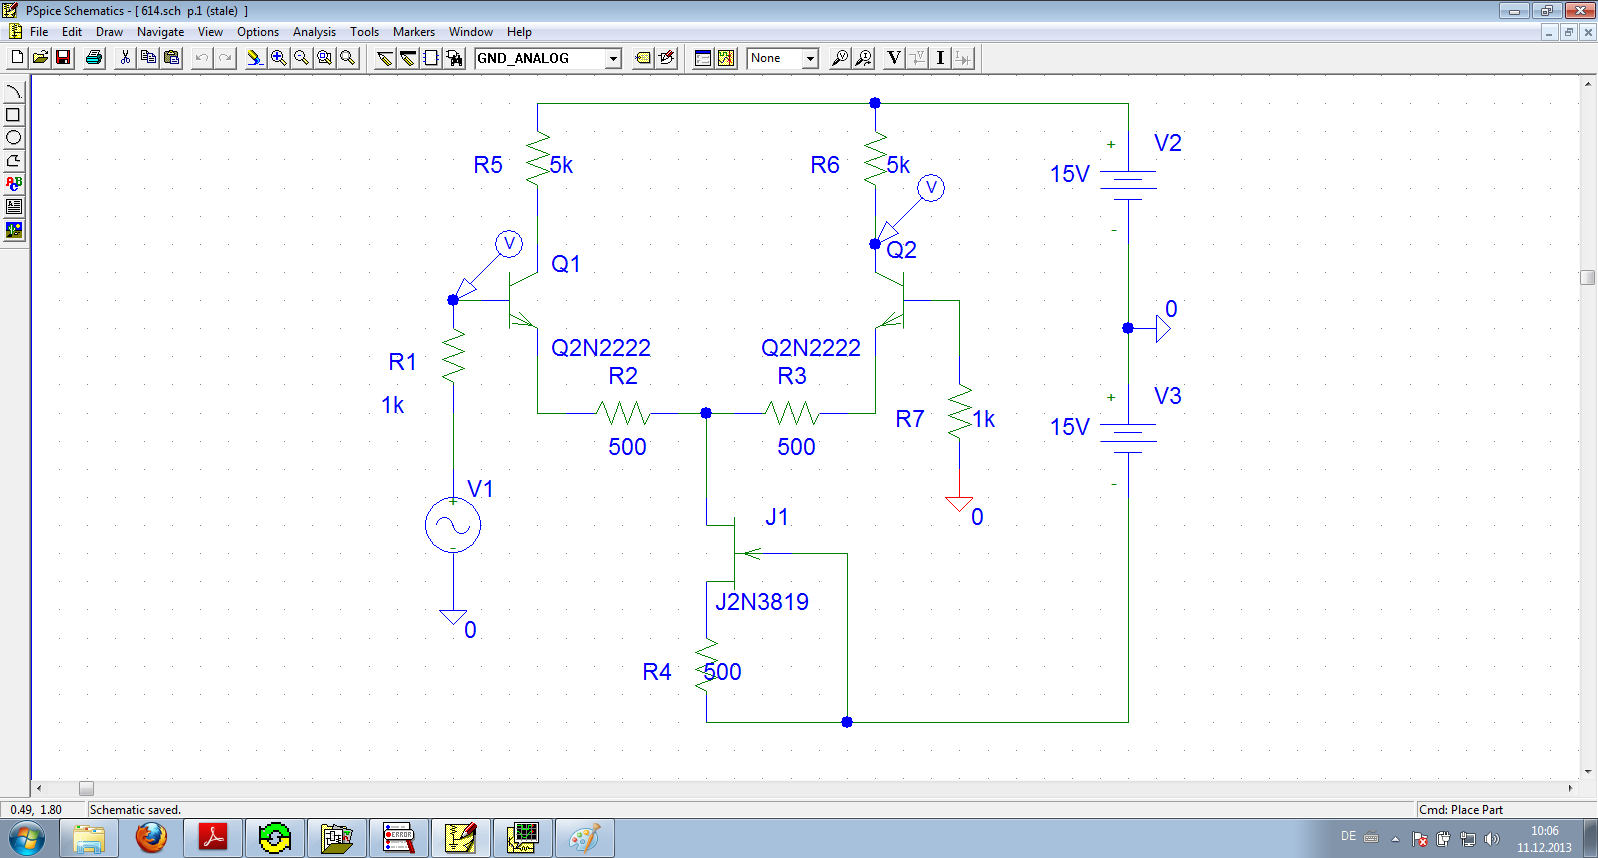
\includegraphics[width=\linewidth]{versuch6/spice/schem614.png}
	\caption{Schaltplan, wie im Skript vorgegeben}
\end{figure}
\begin{figure}[H]
	\centering
	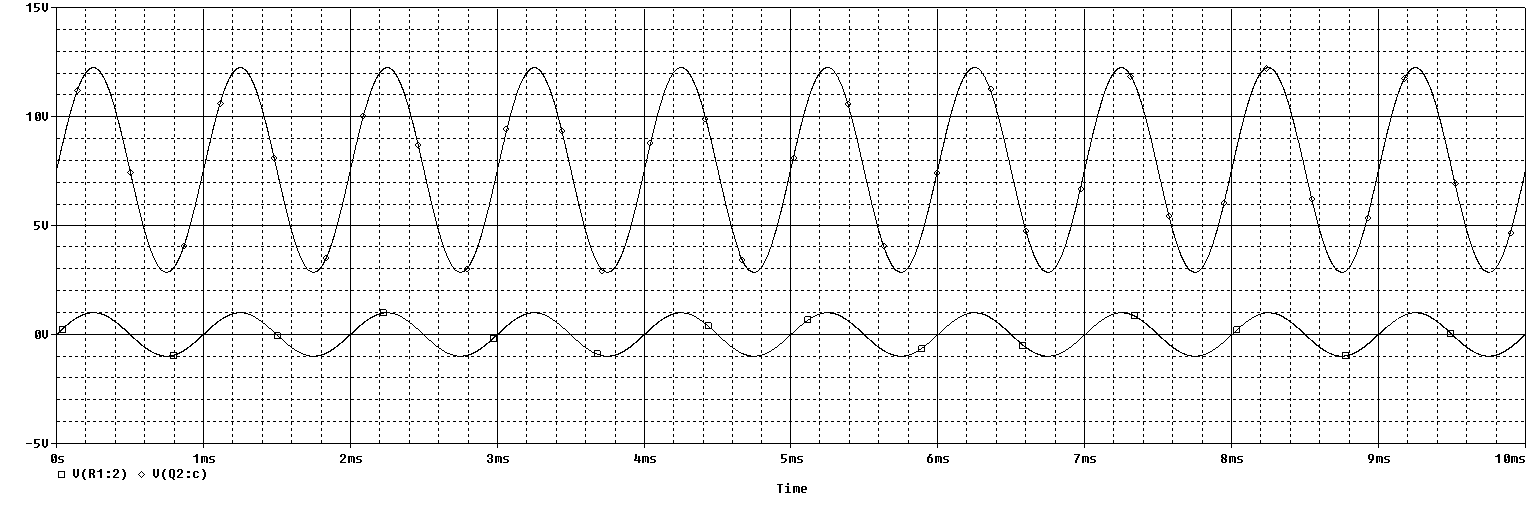
\includegraphics[width=\linewidth]{versuch6/spice/614.png}
	\caption{Simulationsergebnis}
\end{figure}
Die Differenzverstärkung wurde zu 4.75 bestimmt.
\begin{figure}[H]
	\centering
	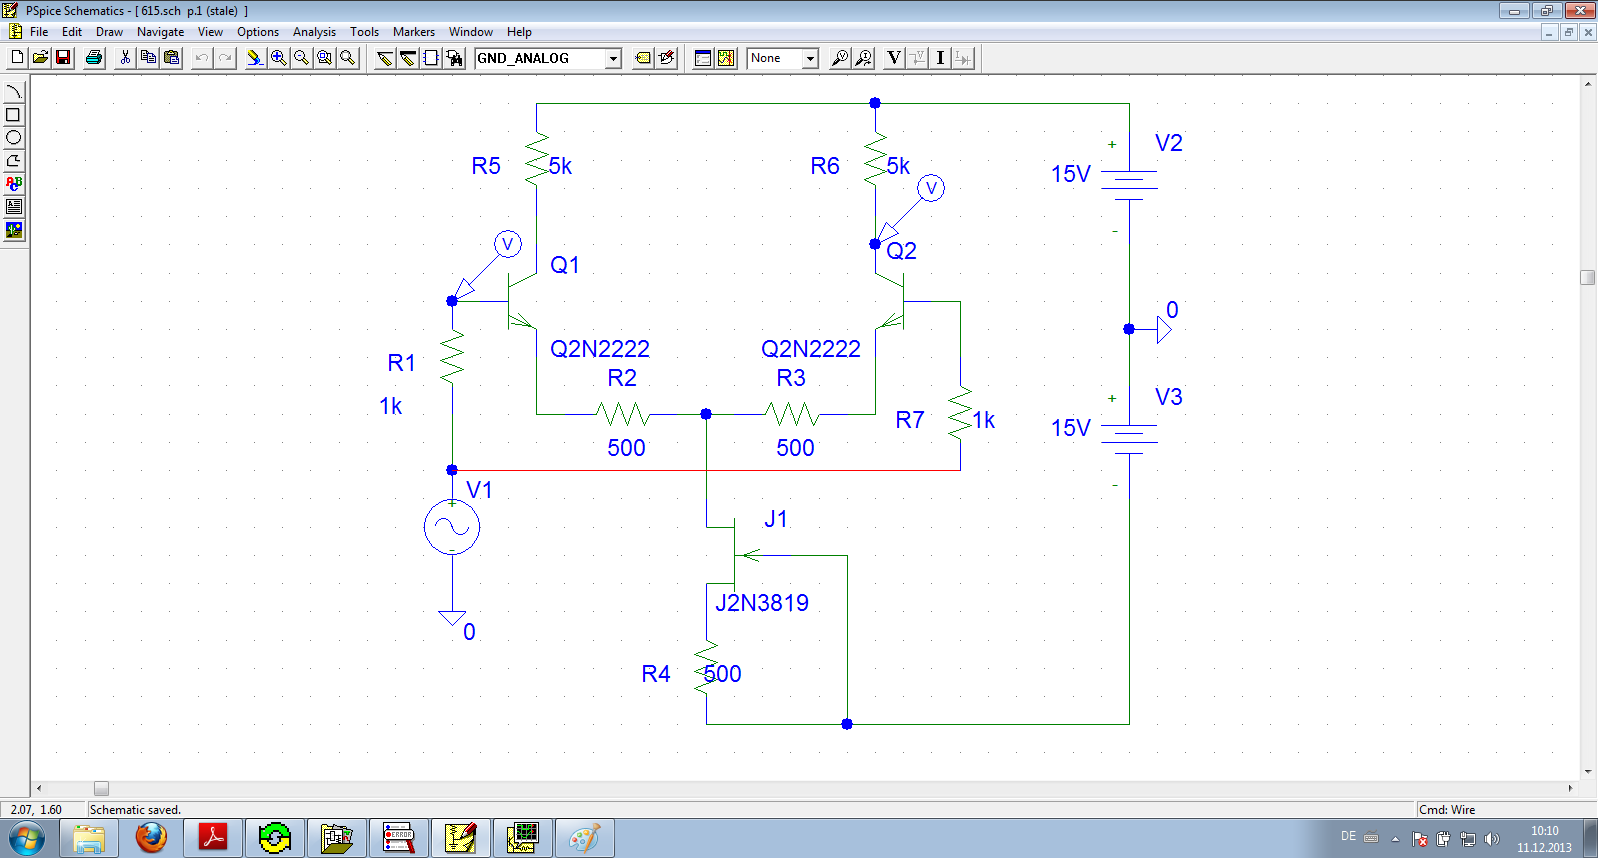
\includegraphics[width=\linewidth]{versuch6/spice/schem615.png}
	\caption{Schaltplan, wie im Skript vorgegeben}
\end{figure}
\begin{figure}[H]
	\centering
	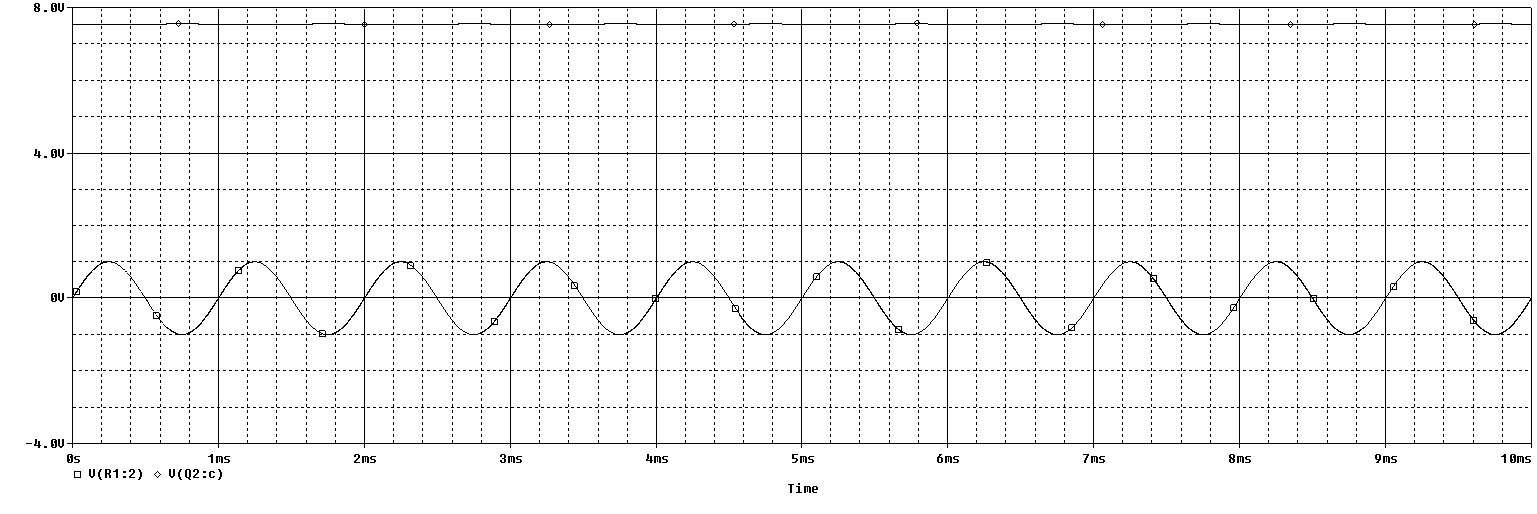
\includegraphics[width=\linewidth]{versuch6/spice/615.png}
	\caption{Simulationsergebnis}
\end{figure}
Die Gleichtaktverstärkung wurde zu 0.005 bestimmt. Damit berechnet sich die Gleichtaktunterdrückung zu $ \frac{4.75}{0.005}=950 $, in Dezibel ergibt dies $ 20*\log_{10}{950} = 59.554 $.\\
Als Nächstes habe ich die Gleichtaktunterdrückung getestet:
\begin{figure}[H]
	\centering
	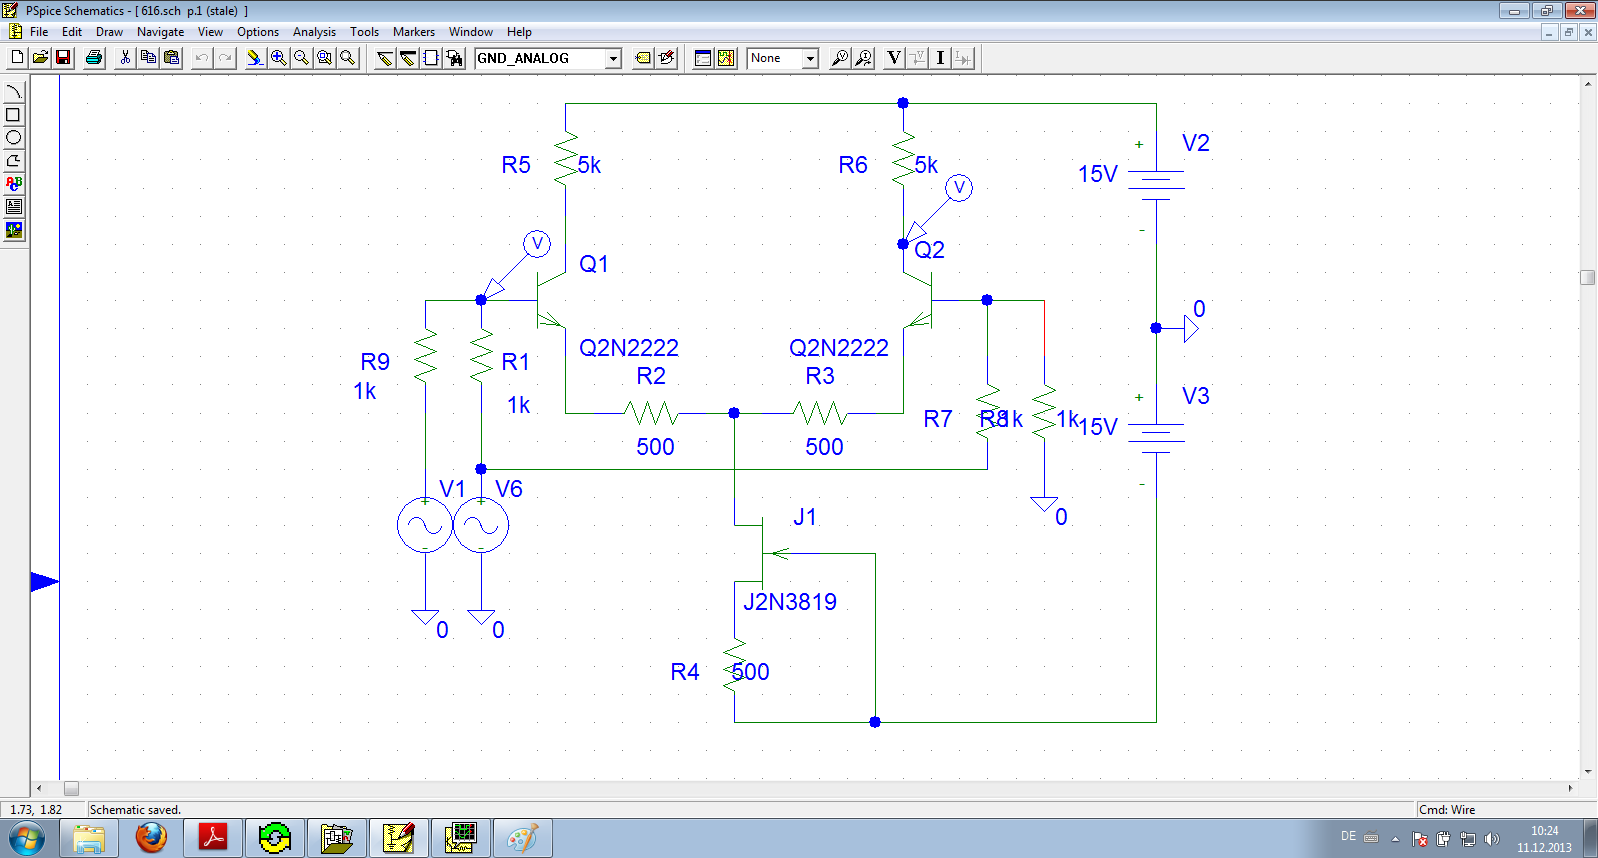
\includegraphics[width=\linewidth]{versuch6/spice/schem616.png}
	\caption{Schaltplan, wie im Skript vorgegeben}
\end{figure}
\begin{figure}[H]
	\centering
	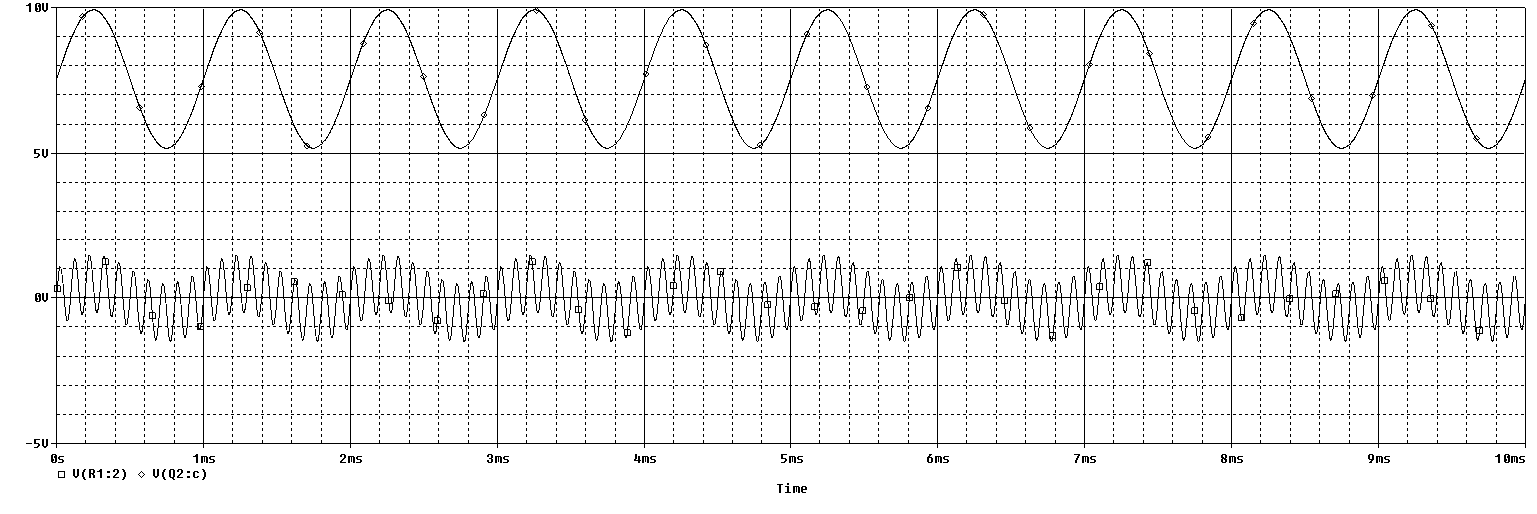
\includegraphics[width=\linewidth]{versuch6/spice/616.png}
	\caption{Simulationsergebnis}
\end{figure}


\subsection{Operationsverstärker als nichtinvertierender Verstärker}
Folgende Schaltung wurde Simuliert:
\begin{figure}[H]
	\centering
	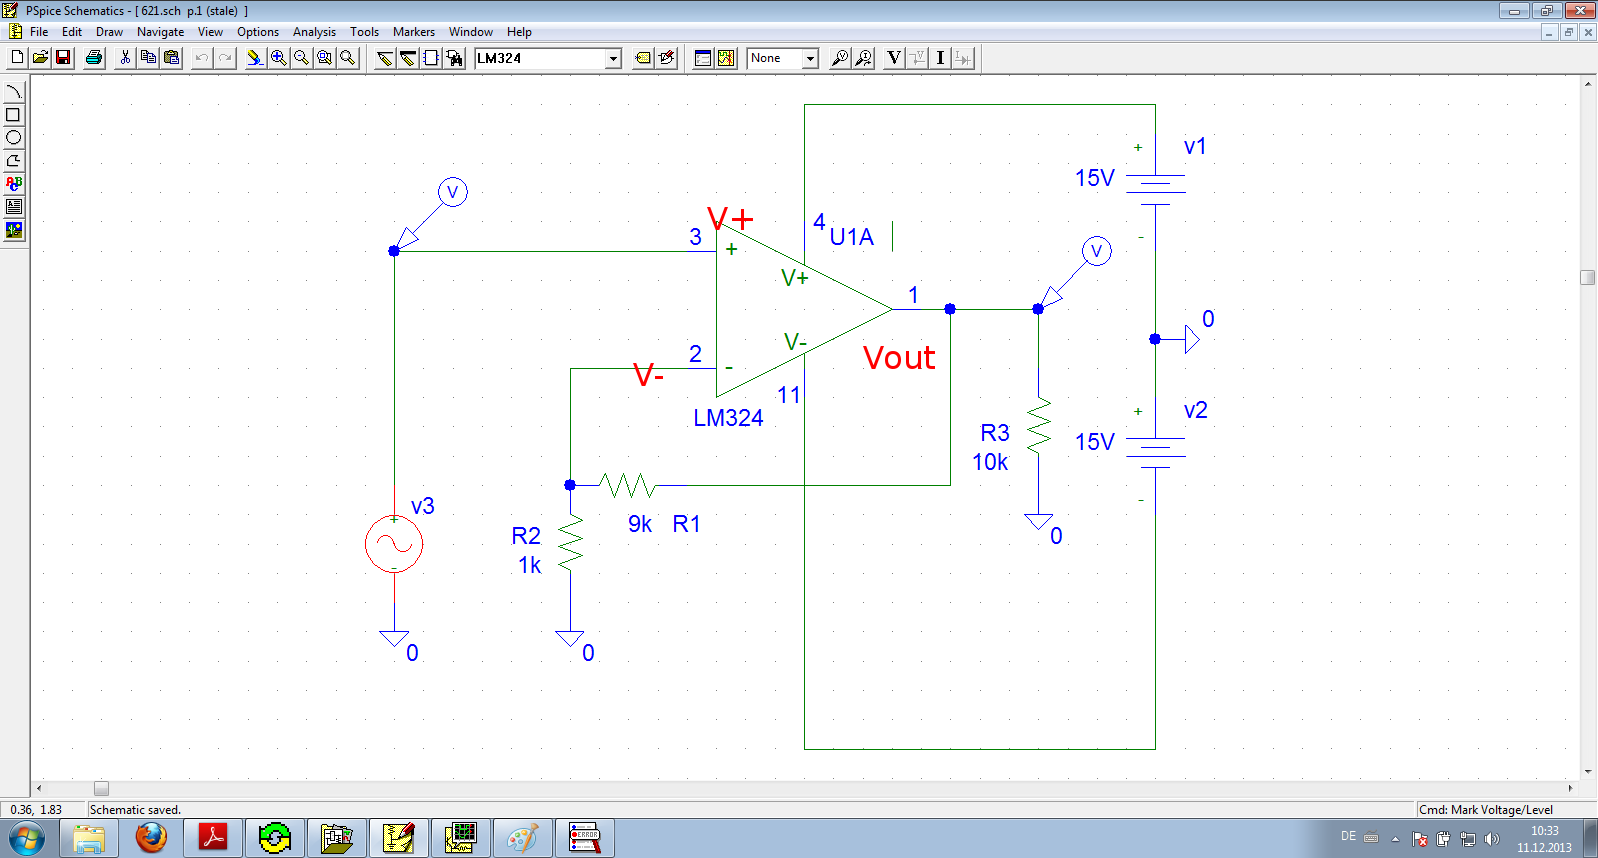
\includegraphics[width=\linewidth]{versuch6/spice/schem621.png}
	\caption{Schaltplan, wie im Skript vorgegeben}
\end{figure}
Damit ergibt sich die Formel für die Ausgangsspannung:\\
Spannungsteiler: $ V_- = V_{out} * \frac{R_2}{R_1+R_2} \Rightarrow V_{out} = V_- * \frac{R_1+R_2}{R_2} $\\
Der Opamp treibt $ V_{out} $ so, dass $ V_+ = V_- \Rightarrow V_{out} = V_+ * \frac{R_1+R_2}{R_2} $ Damit ergibt sich die Verstärkung zu: $ \frac{R_1+R_2}{R_2} = \frac{R_1}{R_2} + \frac{R_1}{R_2} = \frac{R_1}{R_2} +1 = \frac{9k}{1k}+1=10$\\
Der Eingangswiderstand ist nahezu unendlich groß.\\
Die Simulation ergab:
\begin{figure}[H]
	\centering
	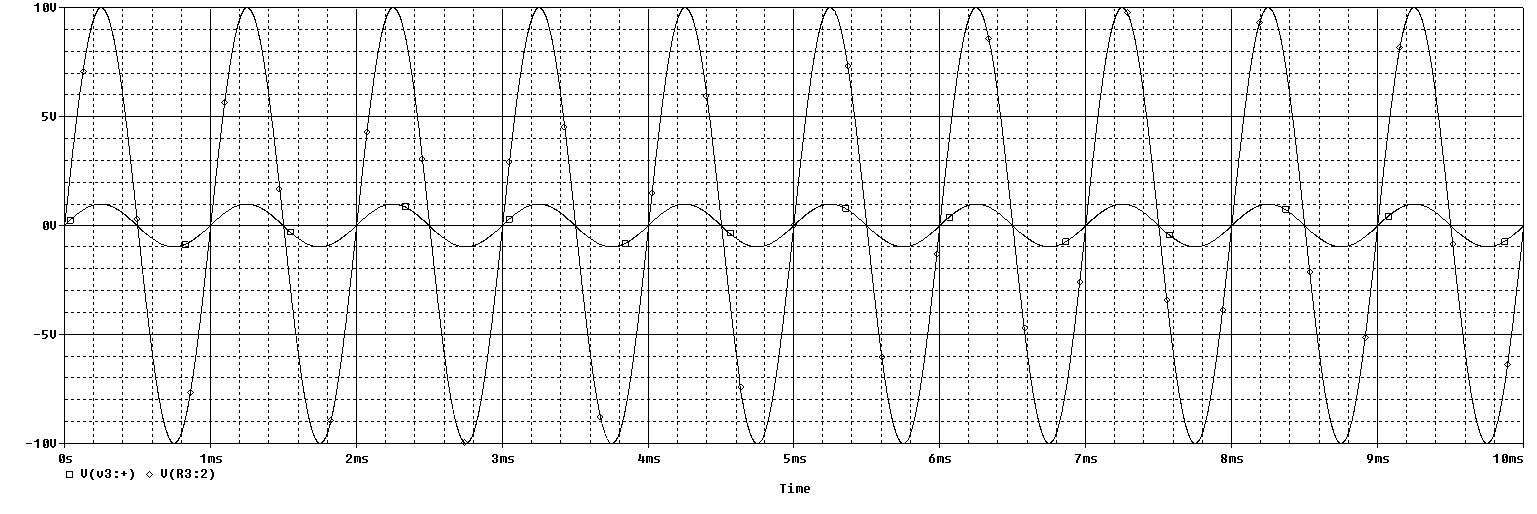
\includegraphics[width=\linewidth]{versuch6/spice/621.png}
	\caption{Simulationsergebnis}
\end{figure}
Mit vergrößerter Spannungsverstärkung ergab sich jedoch:
\begin{figure}[H]
	\centering
	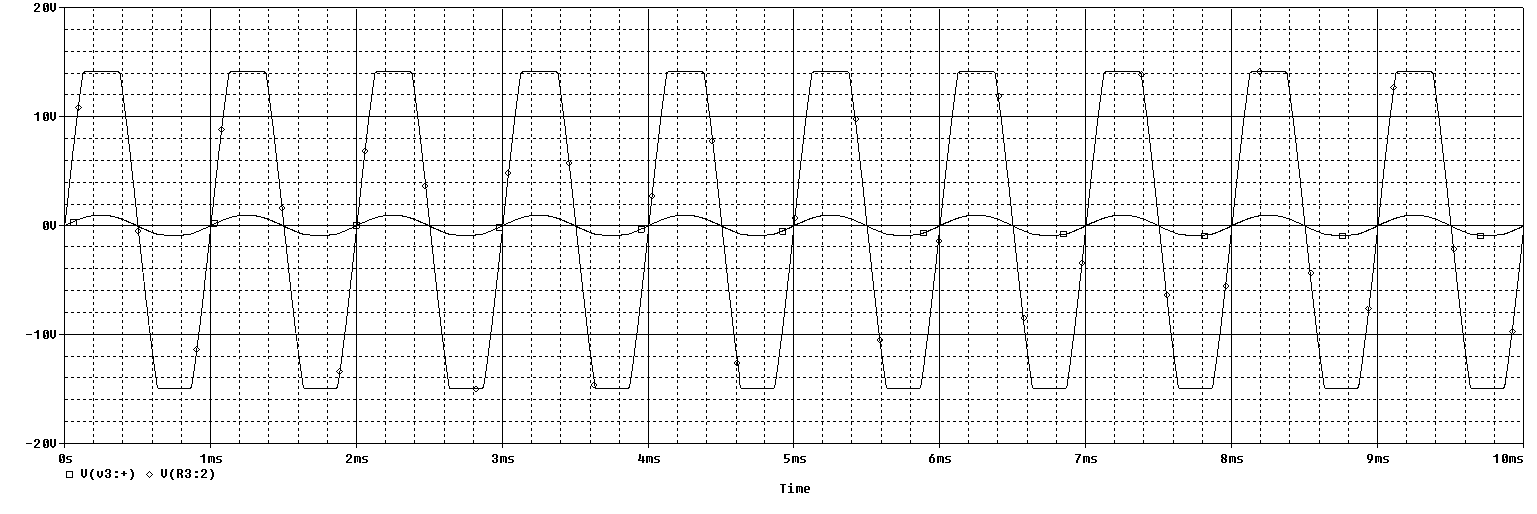
\includegraphics[width=\linewidth]{versuch6/spice/622.png}
	\caption{Simulationsergebnis}
\end{figure}
Man sieht deutlich, dass Clipping eintritt. Der Verstärker kann also die Spannung nicht in den erwünschten Bereich treiben.
\begin{figure}[H]
	\centering
	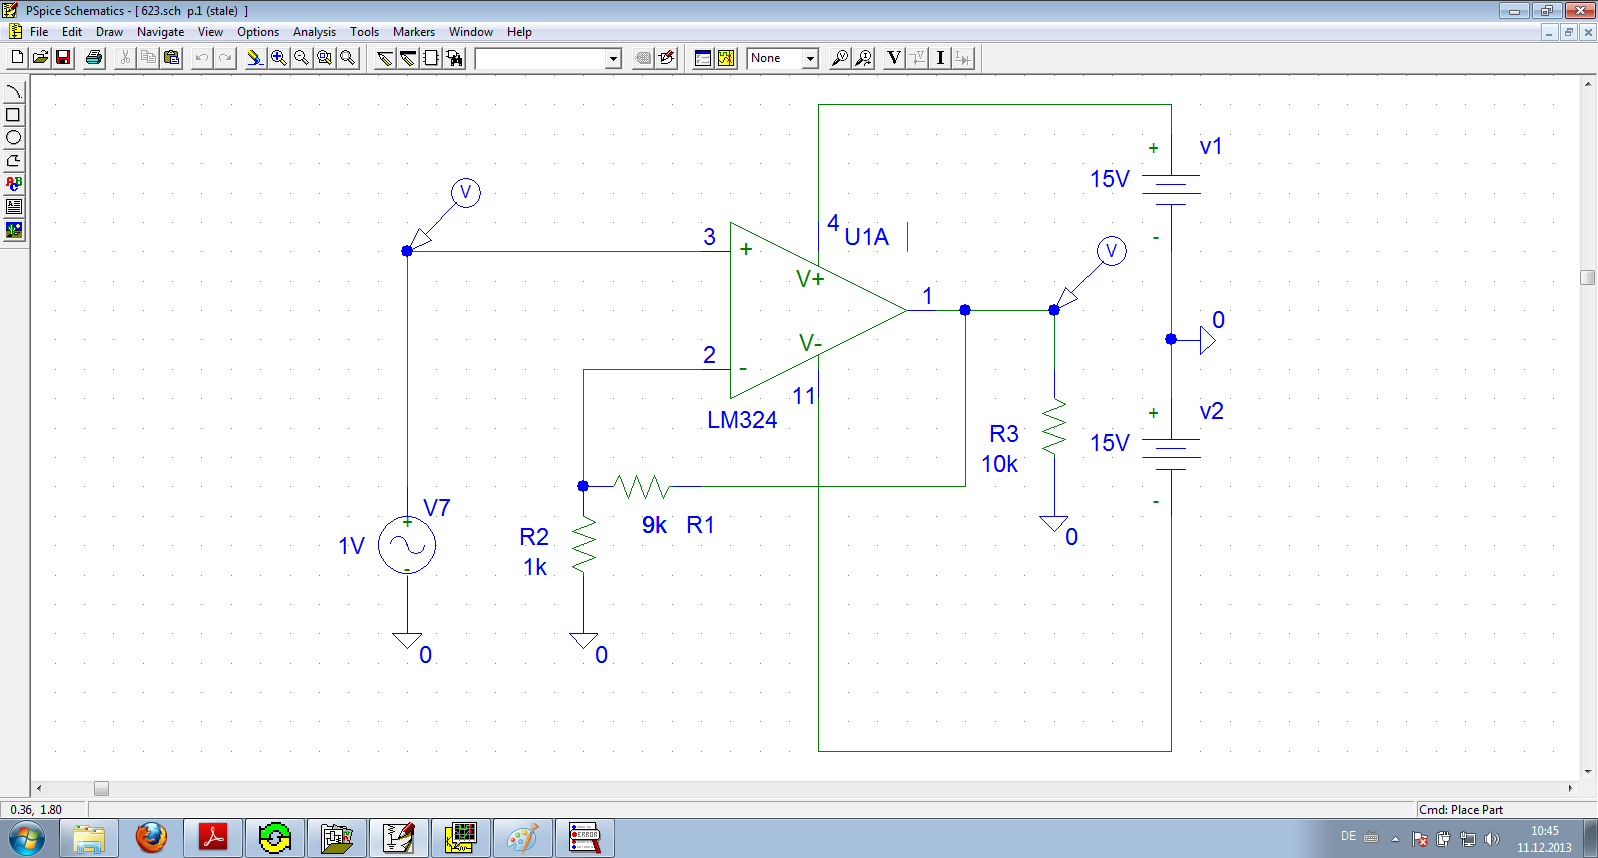
\includegraphics[width=\linewidth]{versuch6/spice/schem623.png}
	\caption{Schaltplan, wie im Skript vorgegeben}
\end{figure}
\begin{figure}[H]
	\centering
	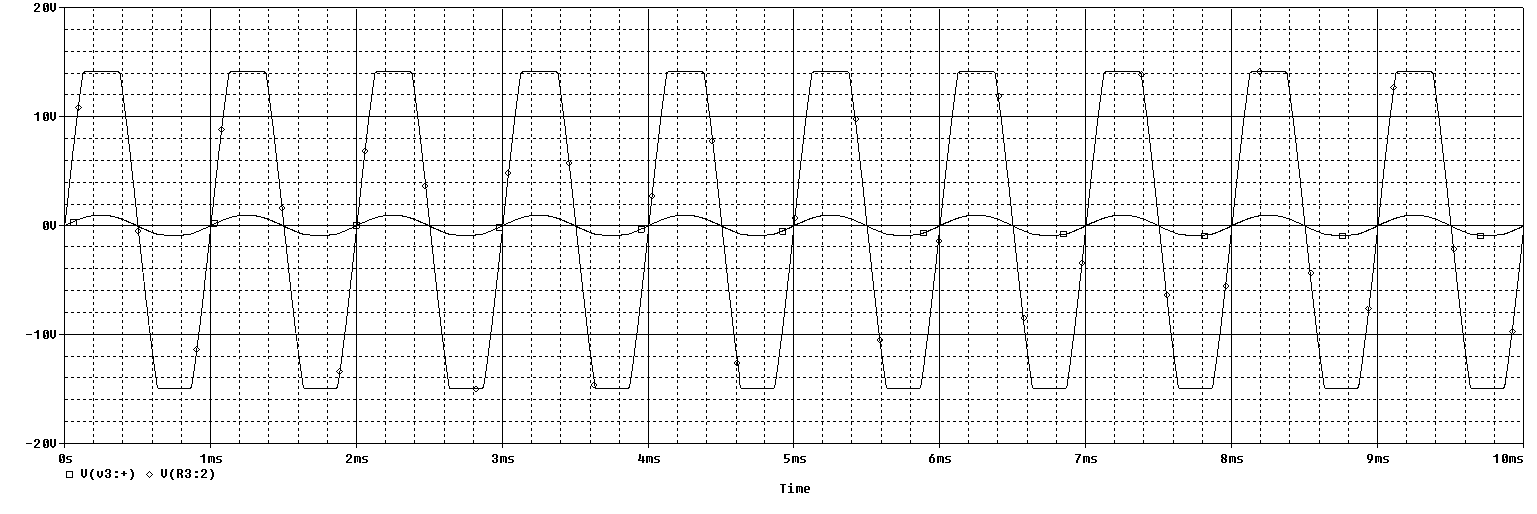
\includegraphics[width=\linewidth]{versuch6/spice/622.png}
	\caption{Simulationsergebnis}
\end{figure}
Die Grenzfrequenz wurde mit der Cursorfunktion auf rund 100kHz bestimmt. Reduziert man hingegen die Spannungsverstärkung auf 2, so erhöht sich die Grenzfrequenz auf 340kHz.% Offensichlich ist der limitierende Faktor die Slewrate des Opamps.

\subsection{Operationsverstärker als invertierender Verstärker}
Folgende Schaltung wurde Simuliert:
\begin{figure}[H]
	\centering
	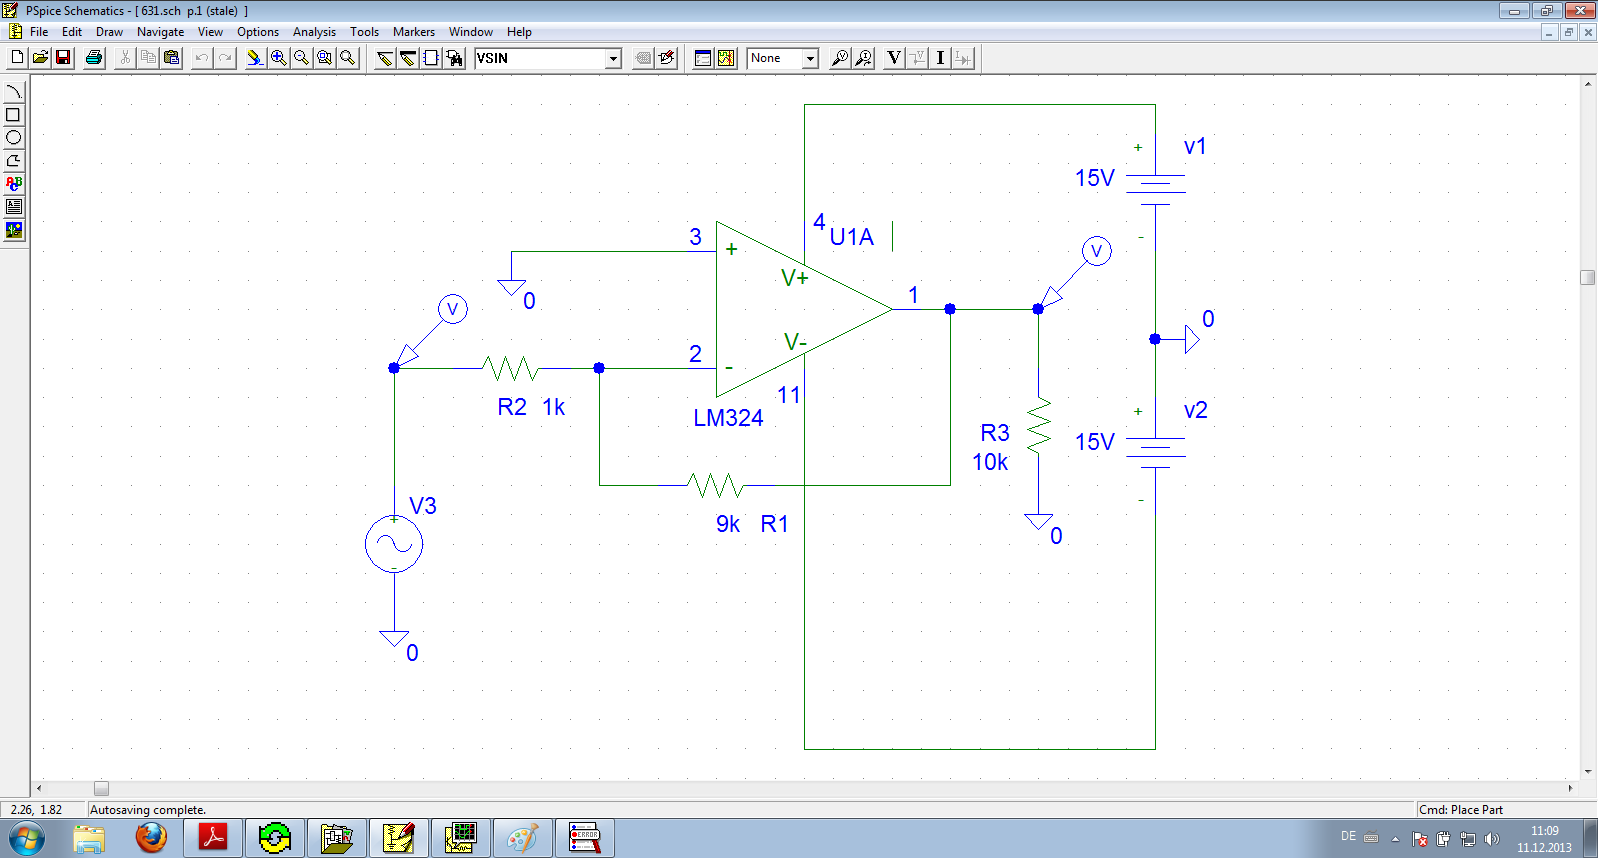
\includegraphics[width=\linewidth]{versuch6/spice/schem631.png}
	\caption{Schaltplan, wie im Skript vorgegeben}
\end{figure}
Auch hier lässt sich die Verstärkung berechnen:\\
Spannungsteiler: $ V_-=\left( \frac{R_2}{R_1+R_2} \left(V_{out}-V_3\right) \right) +V_3 $\\
Der Opamp treibt den Ausgang, sodass die Differenz der Eingänge ist gegen Null geht: \[ V_-=V_+=0 \Rightarrow -V_3 = \frac{R_2}{R_1+R_2} \left(V_{out}-V_3\right) \Rightarrow \left( \frac{R_2}{R_1+R_2} -1 \right) V_3 = \frac{R_2}{R_1+R_2} V_{out}\]
\[\Rightarrow \left(1-\frac{R_1+R_2}{R_2}\right)V_3=V_{out} \Rightarrow \frac{-R_1}{R_2}V_3 = V_{out} \]
Somit beträgt die Spannungsverstärkung $ \frac{-R_1}{R_2} = \frac{-9k\Ohm}{1k\Ohm} = -9 $.\\
Der Eingangswiderstand der Schaltung ist 10k\Ohm, da der Strom durch $ R_2 $ und $ R_1 $ abfließen muss.
\begin{figure}[H]
	\centering
	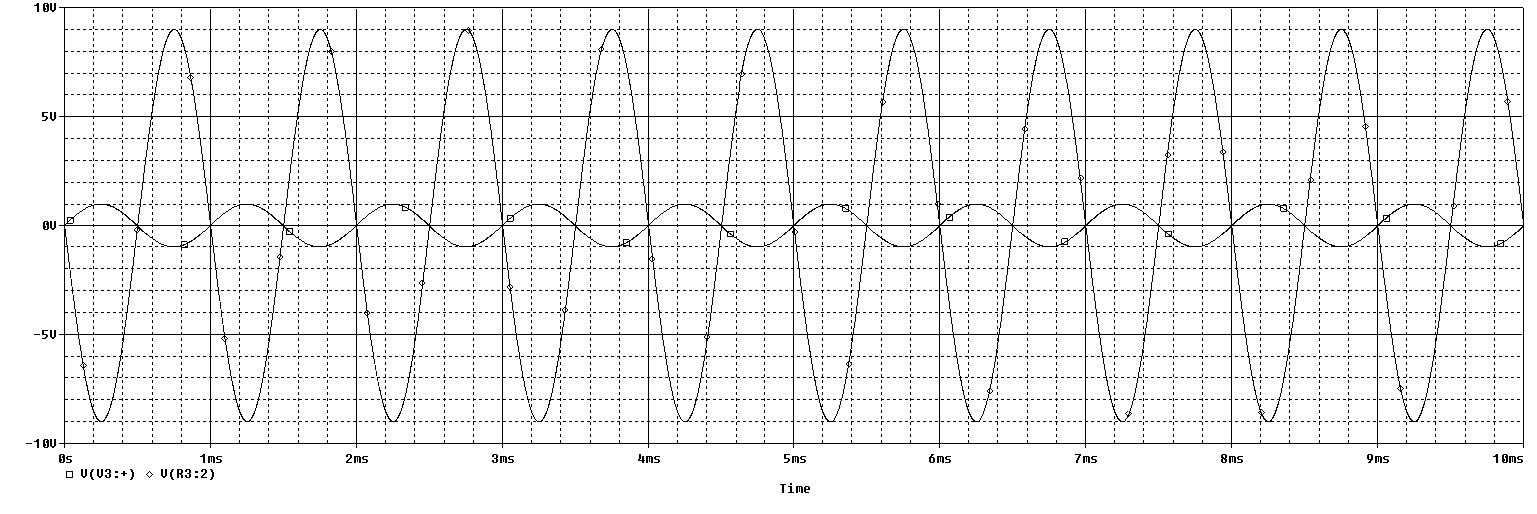
\includegraphics[width=\linewidth]{versuch6/spice/631.png}
	\caption{Simulationsergebnis}
\end{figure}
Die Simulation bestätigt die erwartete Spannungsverstärkung.\\
Nun habe ich die Frequenz auf 100kHz erhöht. Nun zeigt sich deutlich, dass die Slewrate des Operationsverstärkers zu gering ist, da das Ausgangssignal zu einer Dreieckschwingung verkommt.
\begin{figure}[H]
	\centering
	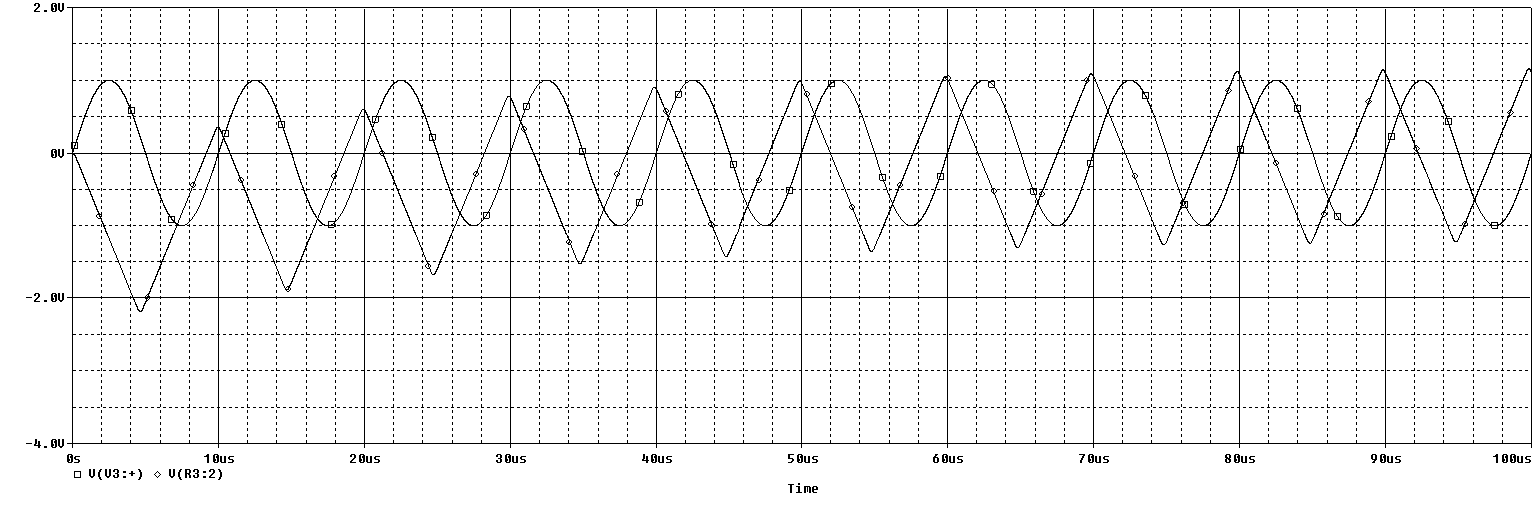
\includegraphics[width=\linewidth]{versuch6/spice/632.png}
	\caption{Simulationsergebnis}
\end{figure}

\subsection{Die realen Schaltungen}
\subsubsection*{Verstärkungsfaktoren}
\paragraph{Der invertierende Verstärker}
\begin{figure}[H]
	\centering
	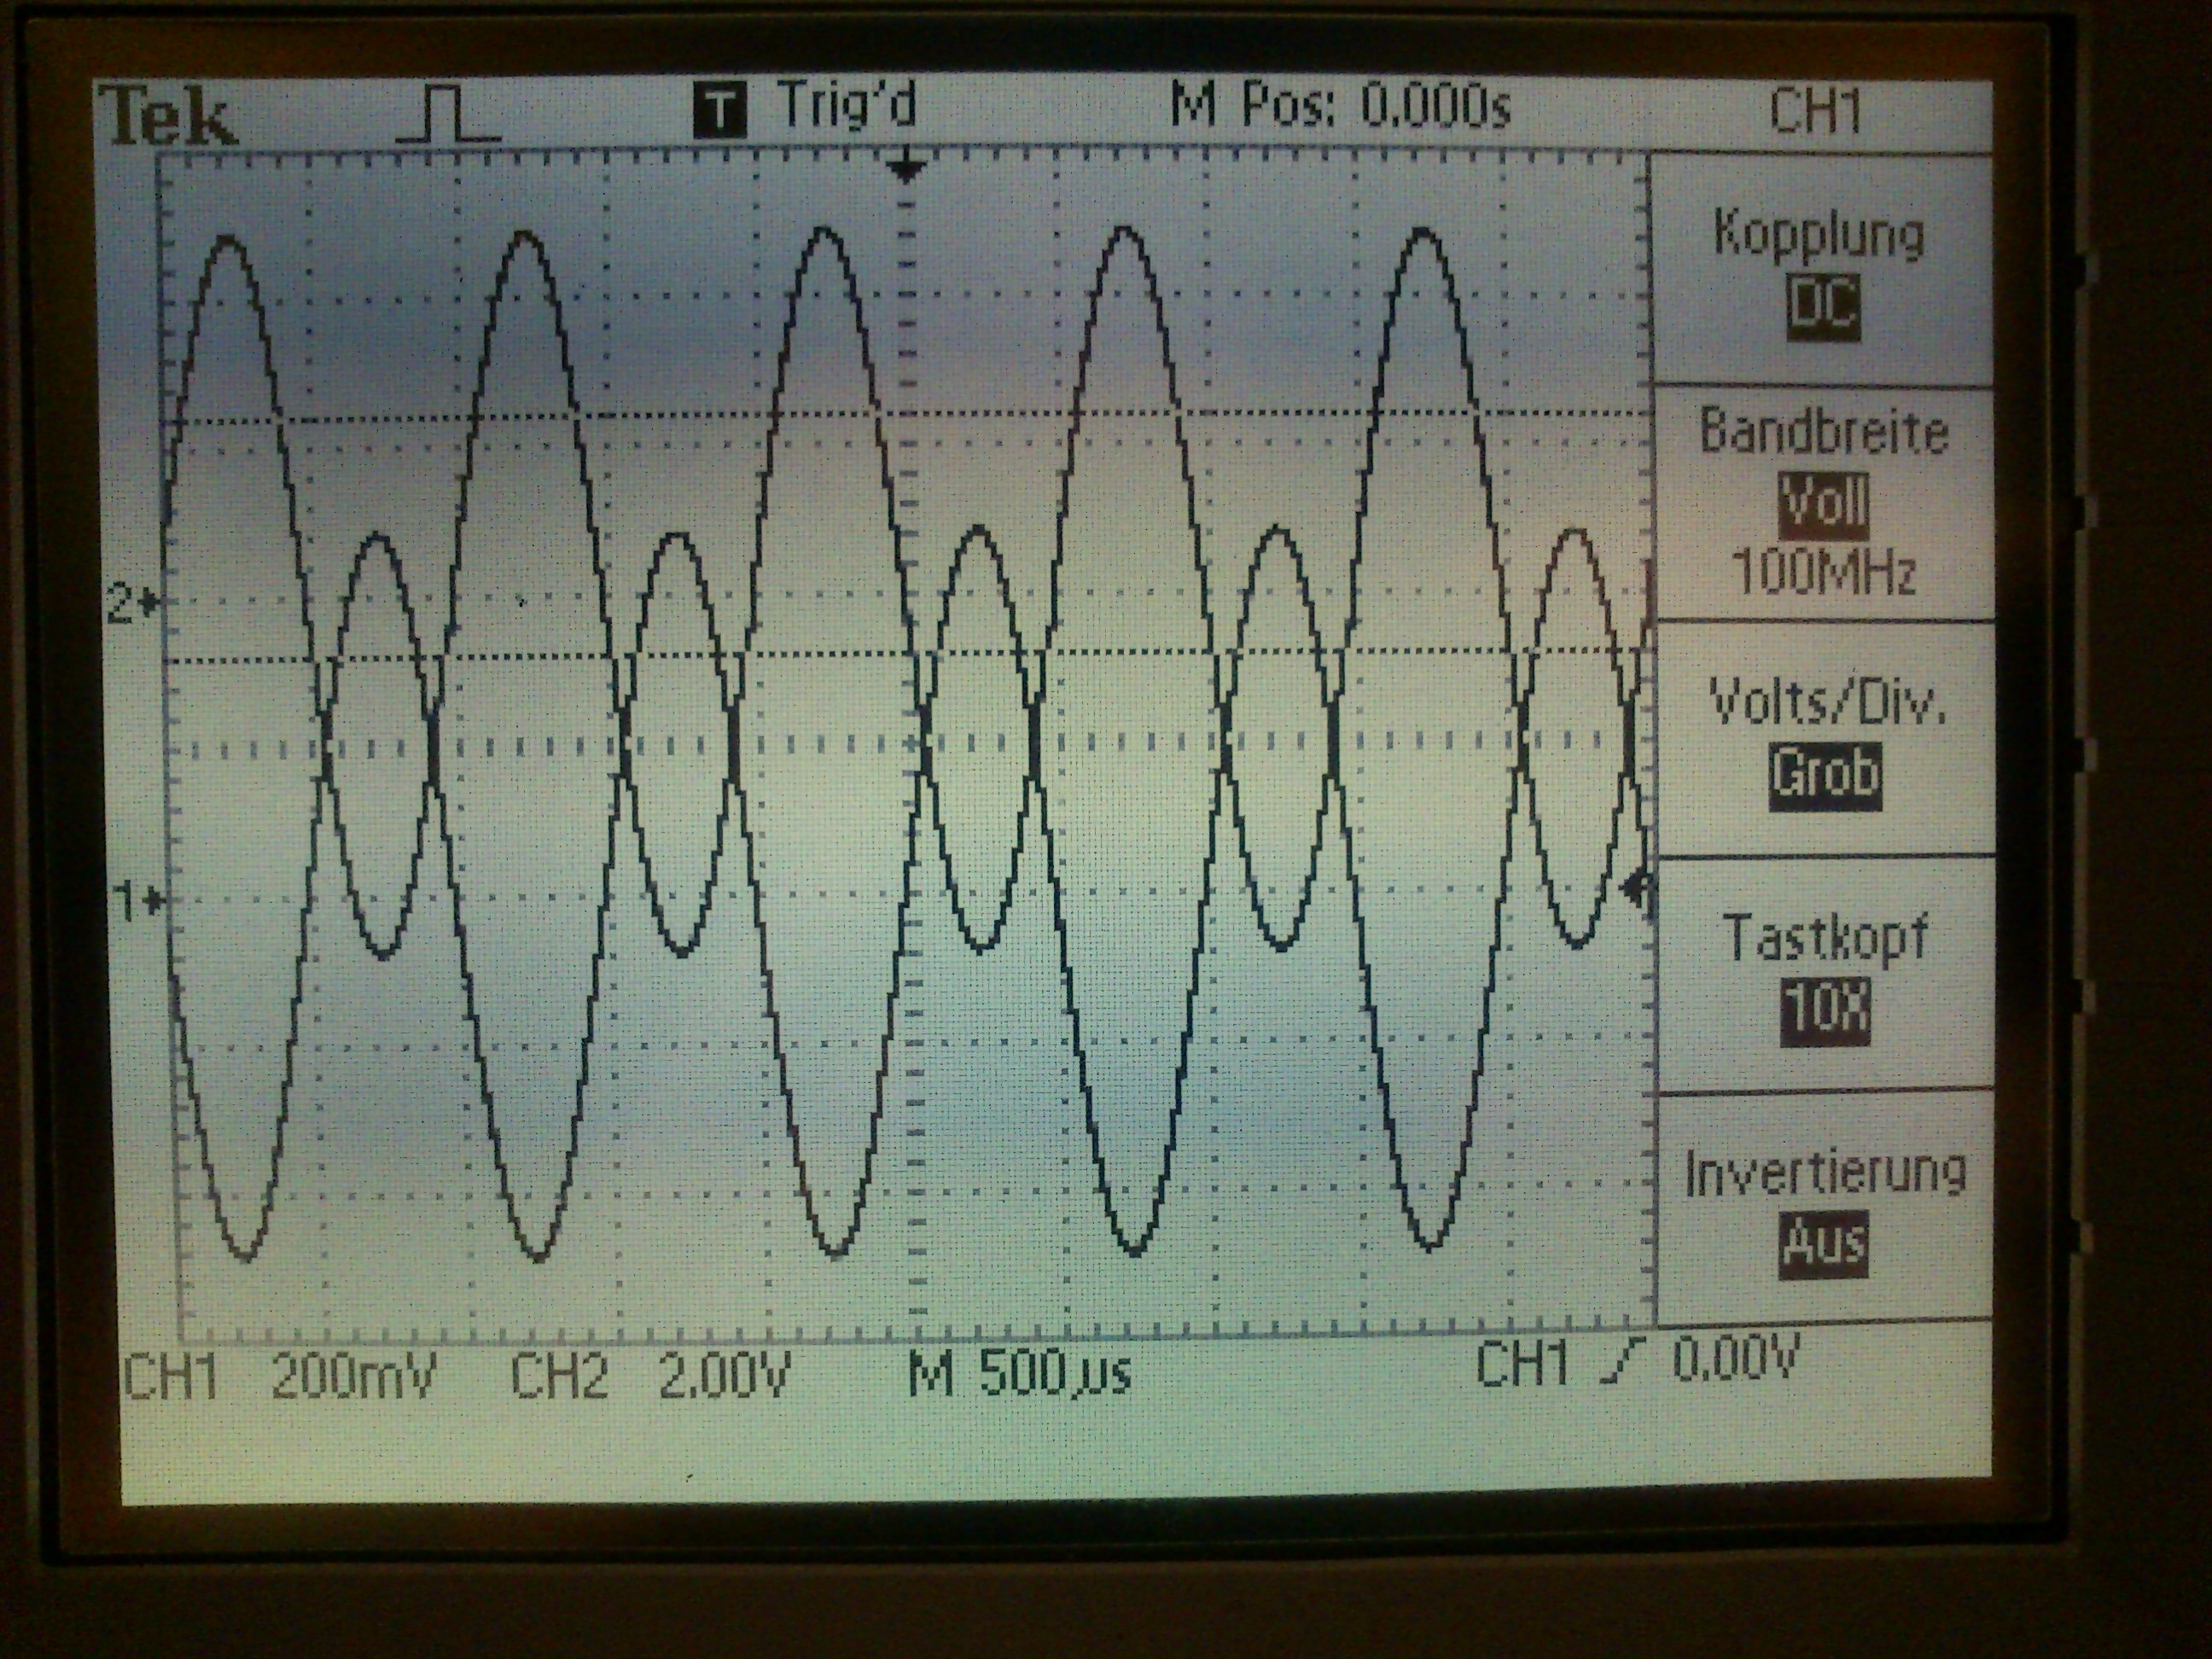
\includegraphics[width=\linewidth]{versuch6/oszi/DSC_0477.JPG}
	\caption{Kanal 1: Eingangsspannung; Kanal 2: Ausgangsspannung}
\end{figure}
Wie man sieht, ist der Verstärkungsfaktor des invertierenden Verstärkers 10.


\paragraph{Der nichtinvertierende Verstärker}
\begin{figure}[H]
	\centering
	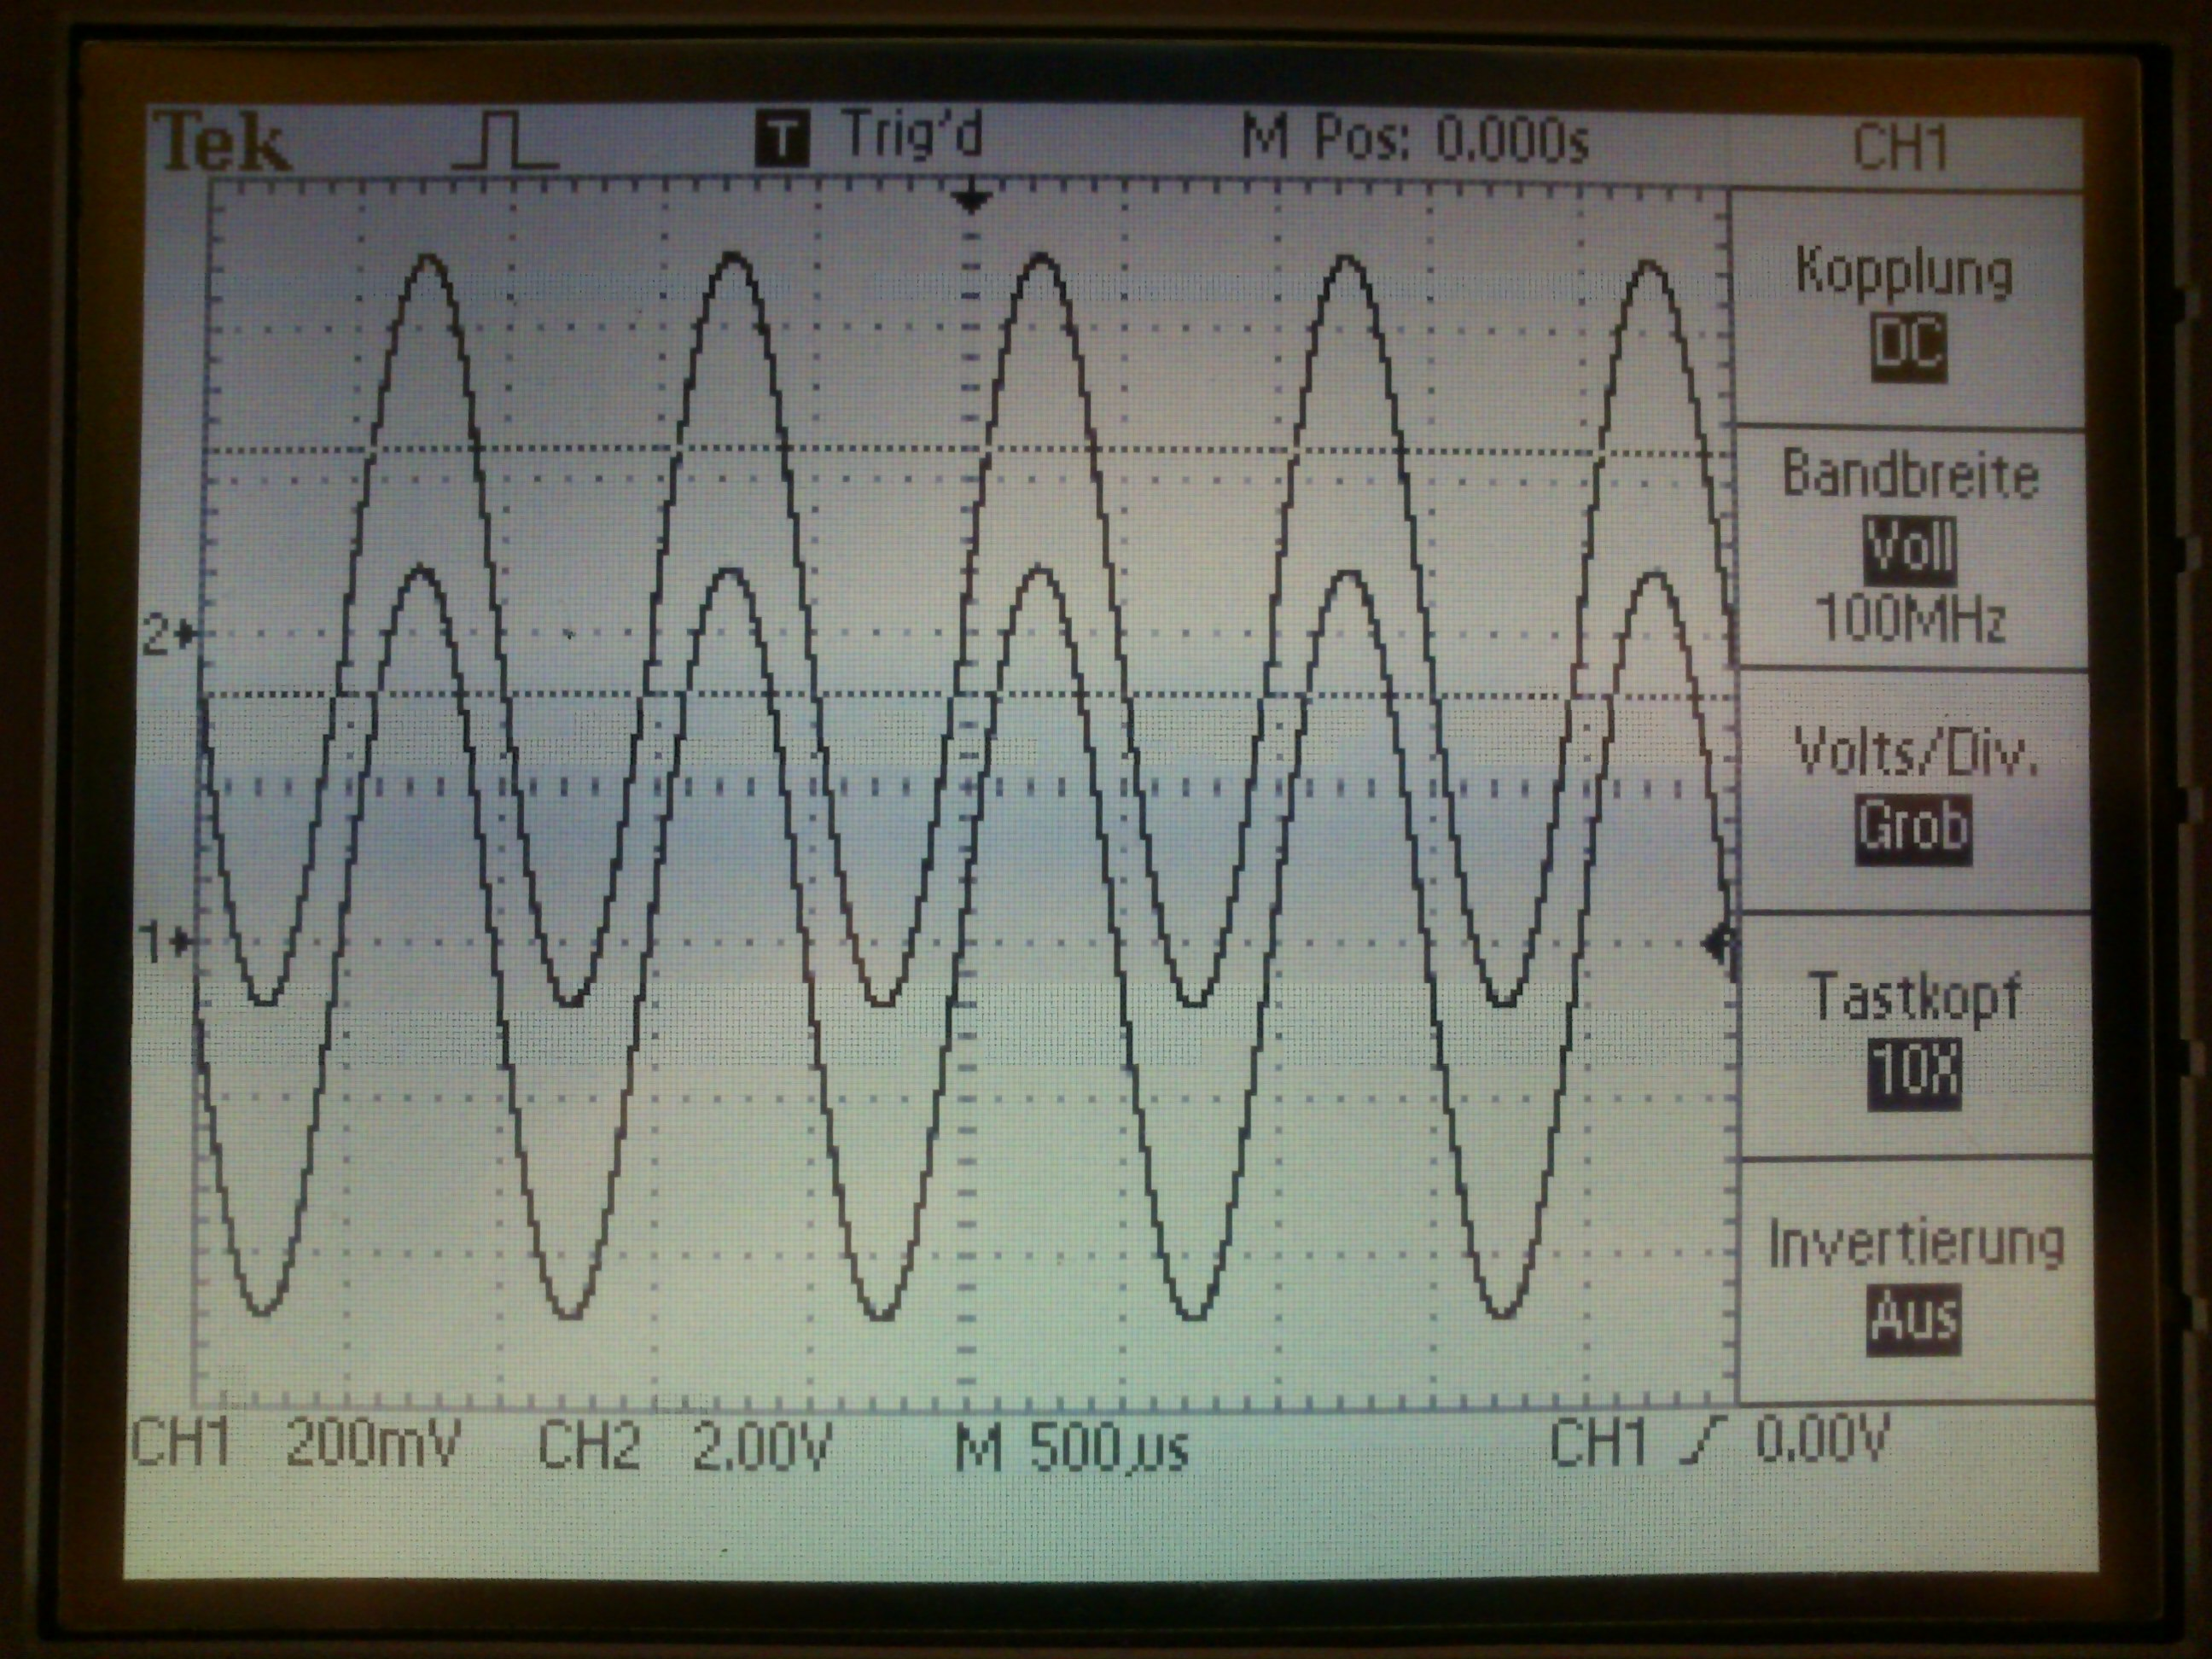
\includegraphics[width=\linewidth]{versuch6/oszi/DSC_0480.JPG}
	\caption{Kanal 1: Eingangsspannung; Kanal 2: Ausgangsspannung}
\end{figure}
Wie man sieht, ist der Verstärkungsfaktor des nichtinvertierenden Verstärkers auch 10.

\subsubsection*{Bandbreite}
\begin{tabular}{l l}
	Verstärkertyp & Bandbreite\\
	invertierend & 60kHz\\
	nichtinvertierend & 60kHz\\
\end{tabular}
Die untere Halbwelle des Ausgangssignals ist abgeflacht, und nur ein kleiner Spike erreicht die untere Scheitelspannung.

\subsubsection*{Slewrate}
\begin{tabular}{l l}
	Verstärkertyp & Slewrate\\
	nichtinvertierend & $ 0.32468 \frac{V}{\µs} $\\
	invertierend & $ 0.3333 \frac{V}{\µs} $\\
\end{tabular}
\begin{figure}[H]
	\centering
	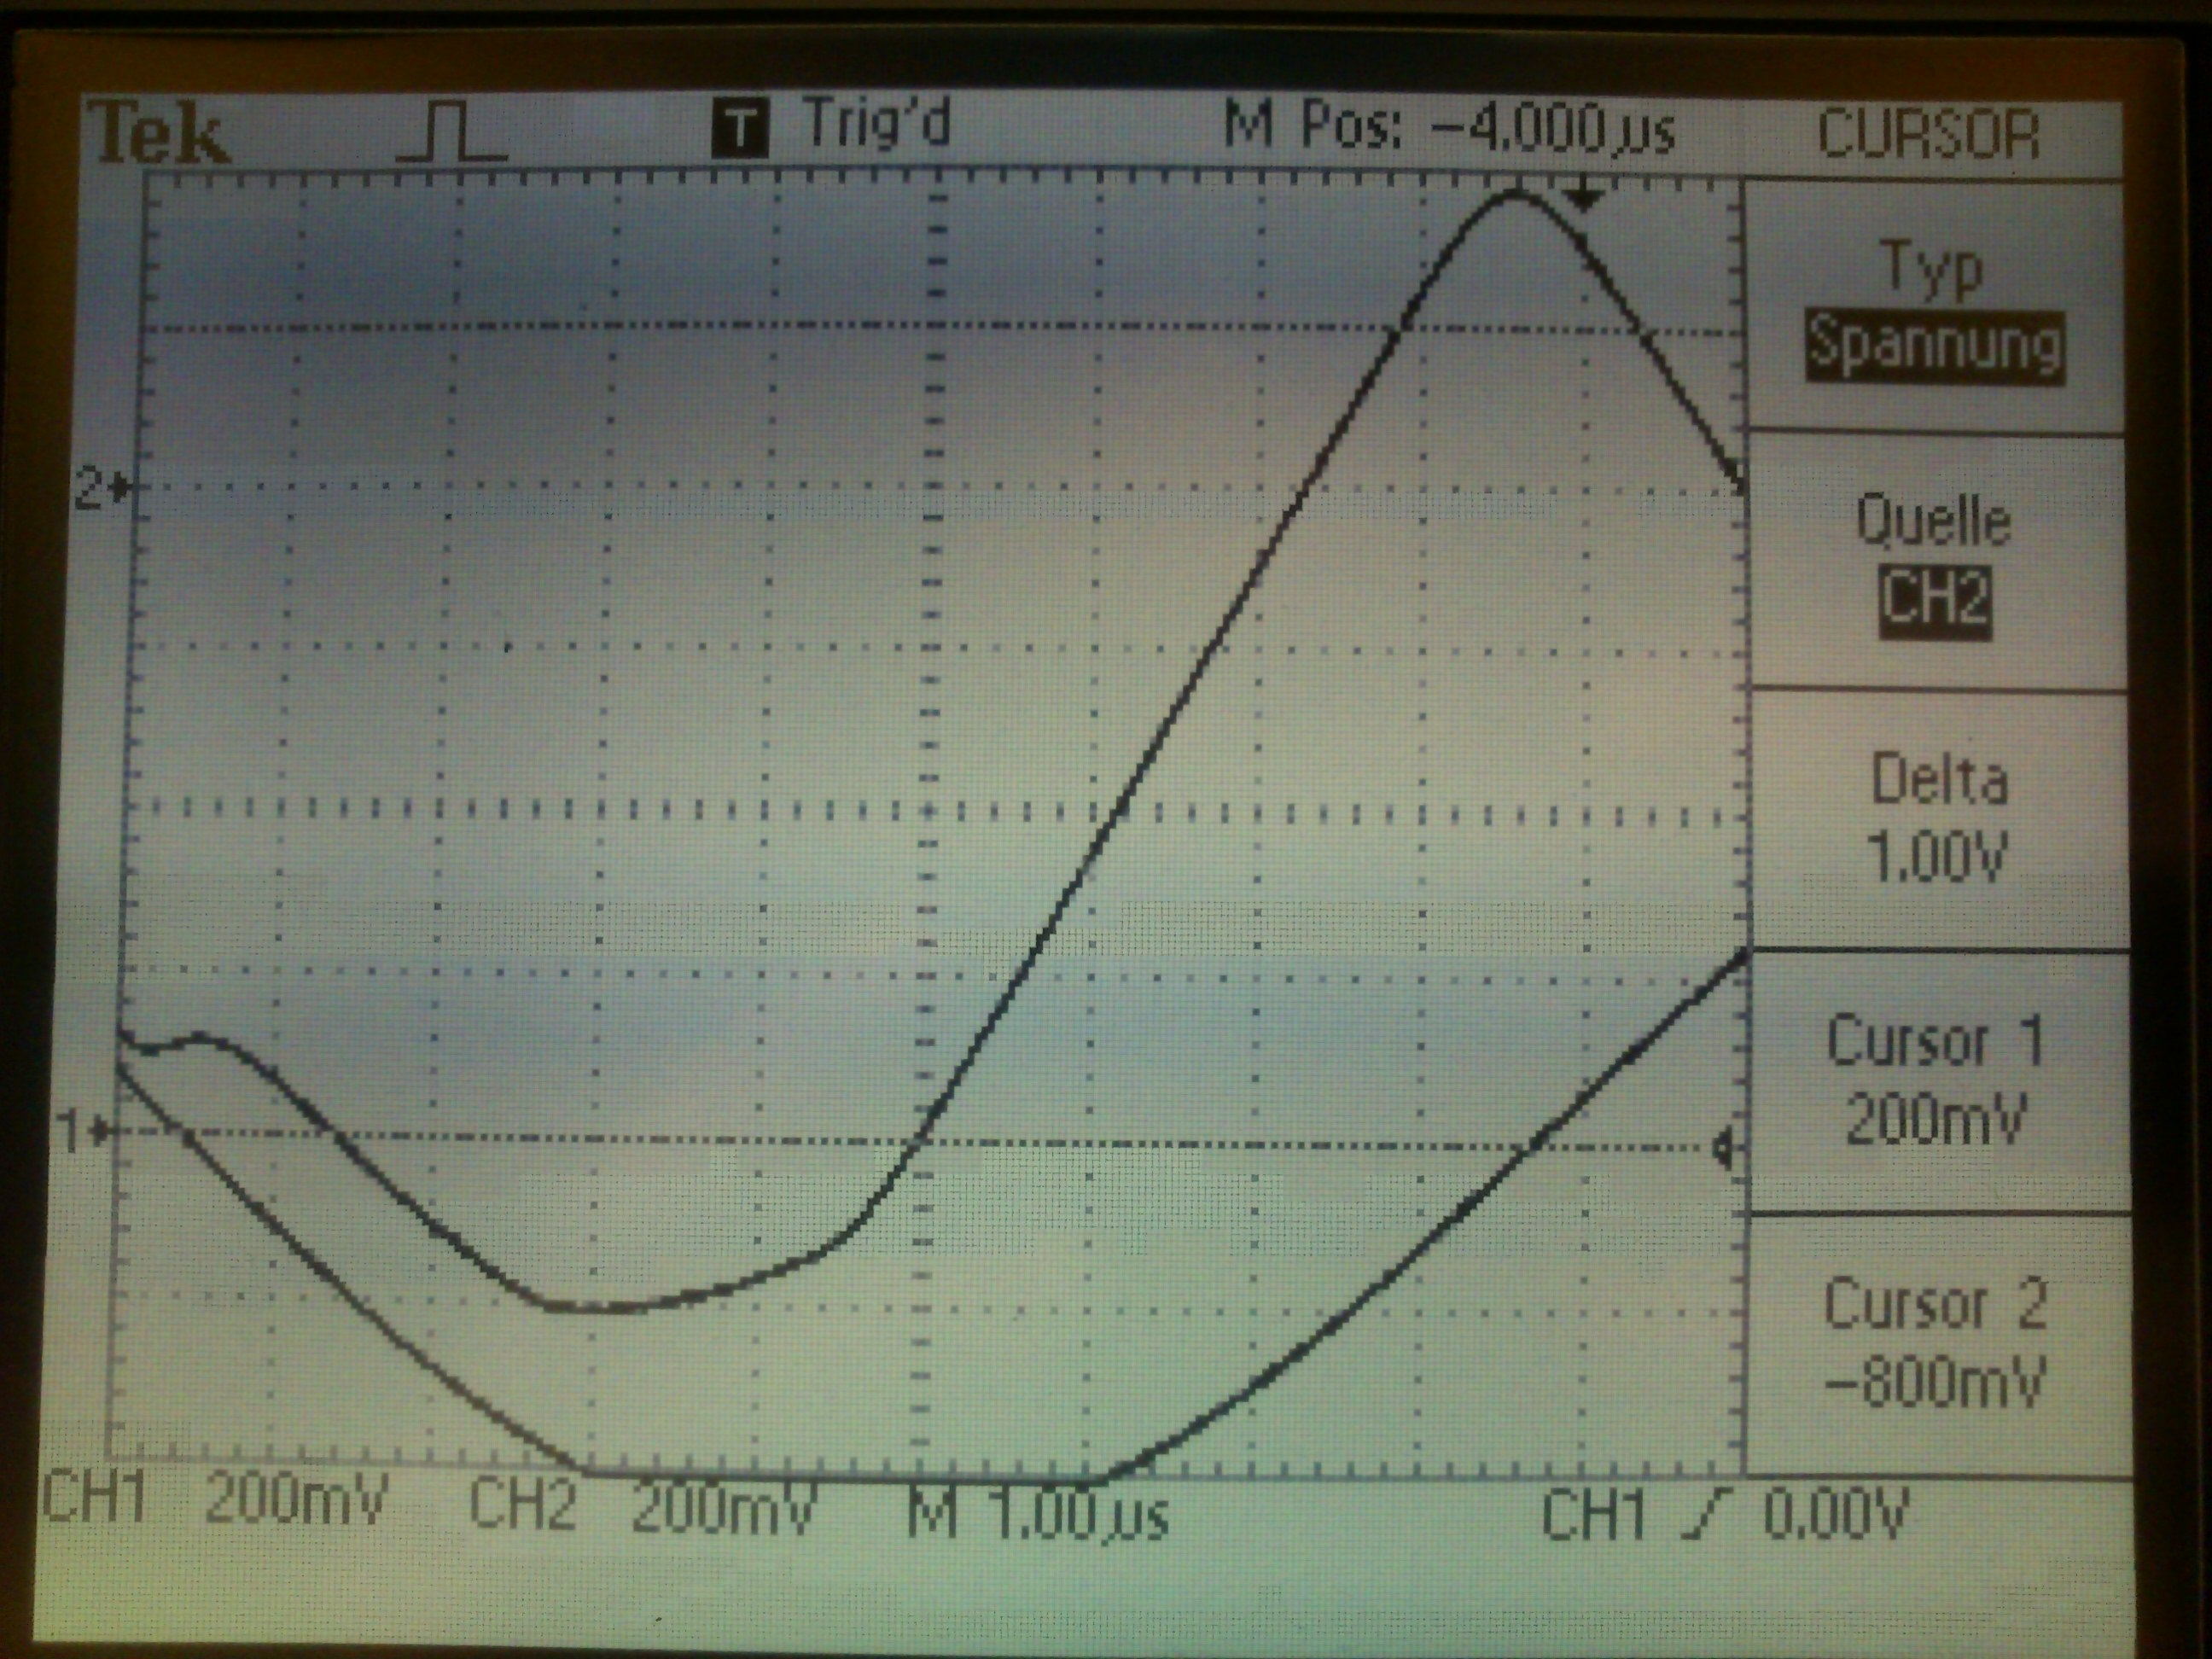
\includegraphics[width=\linewidth]{versuch6/oszi/DSC_0501.JPG}
	\caption{Bestimmung am nichtinvertierenden Verstärker}
\end{figure}
\begin{figure}[H]
	\centering
	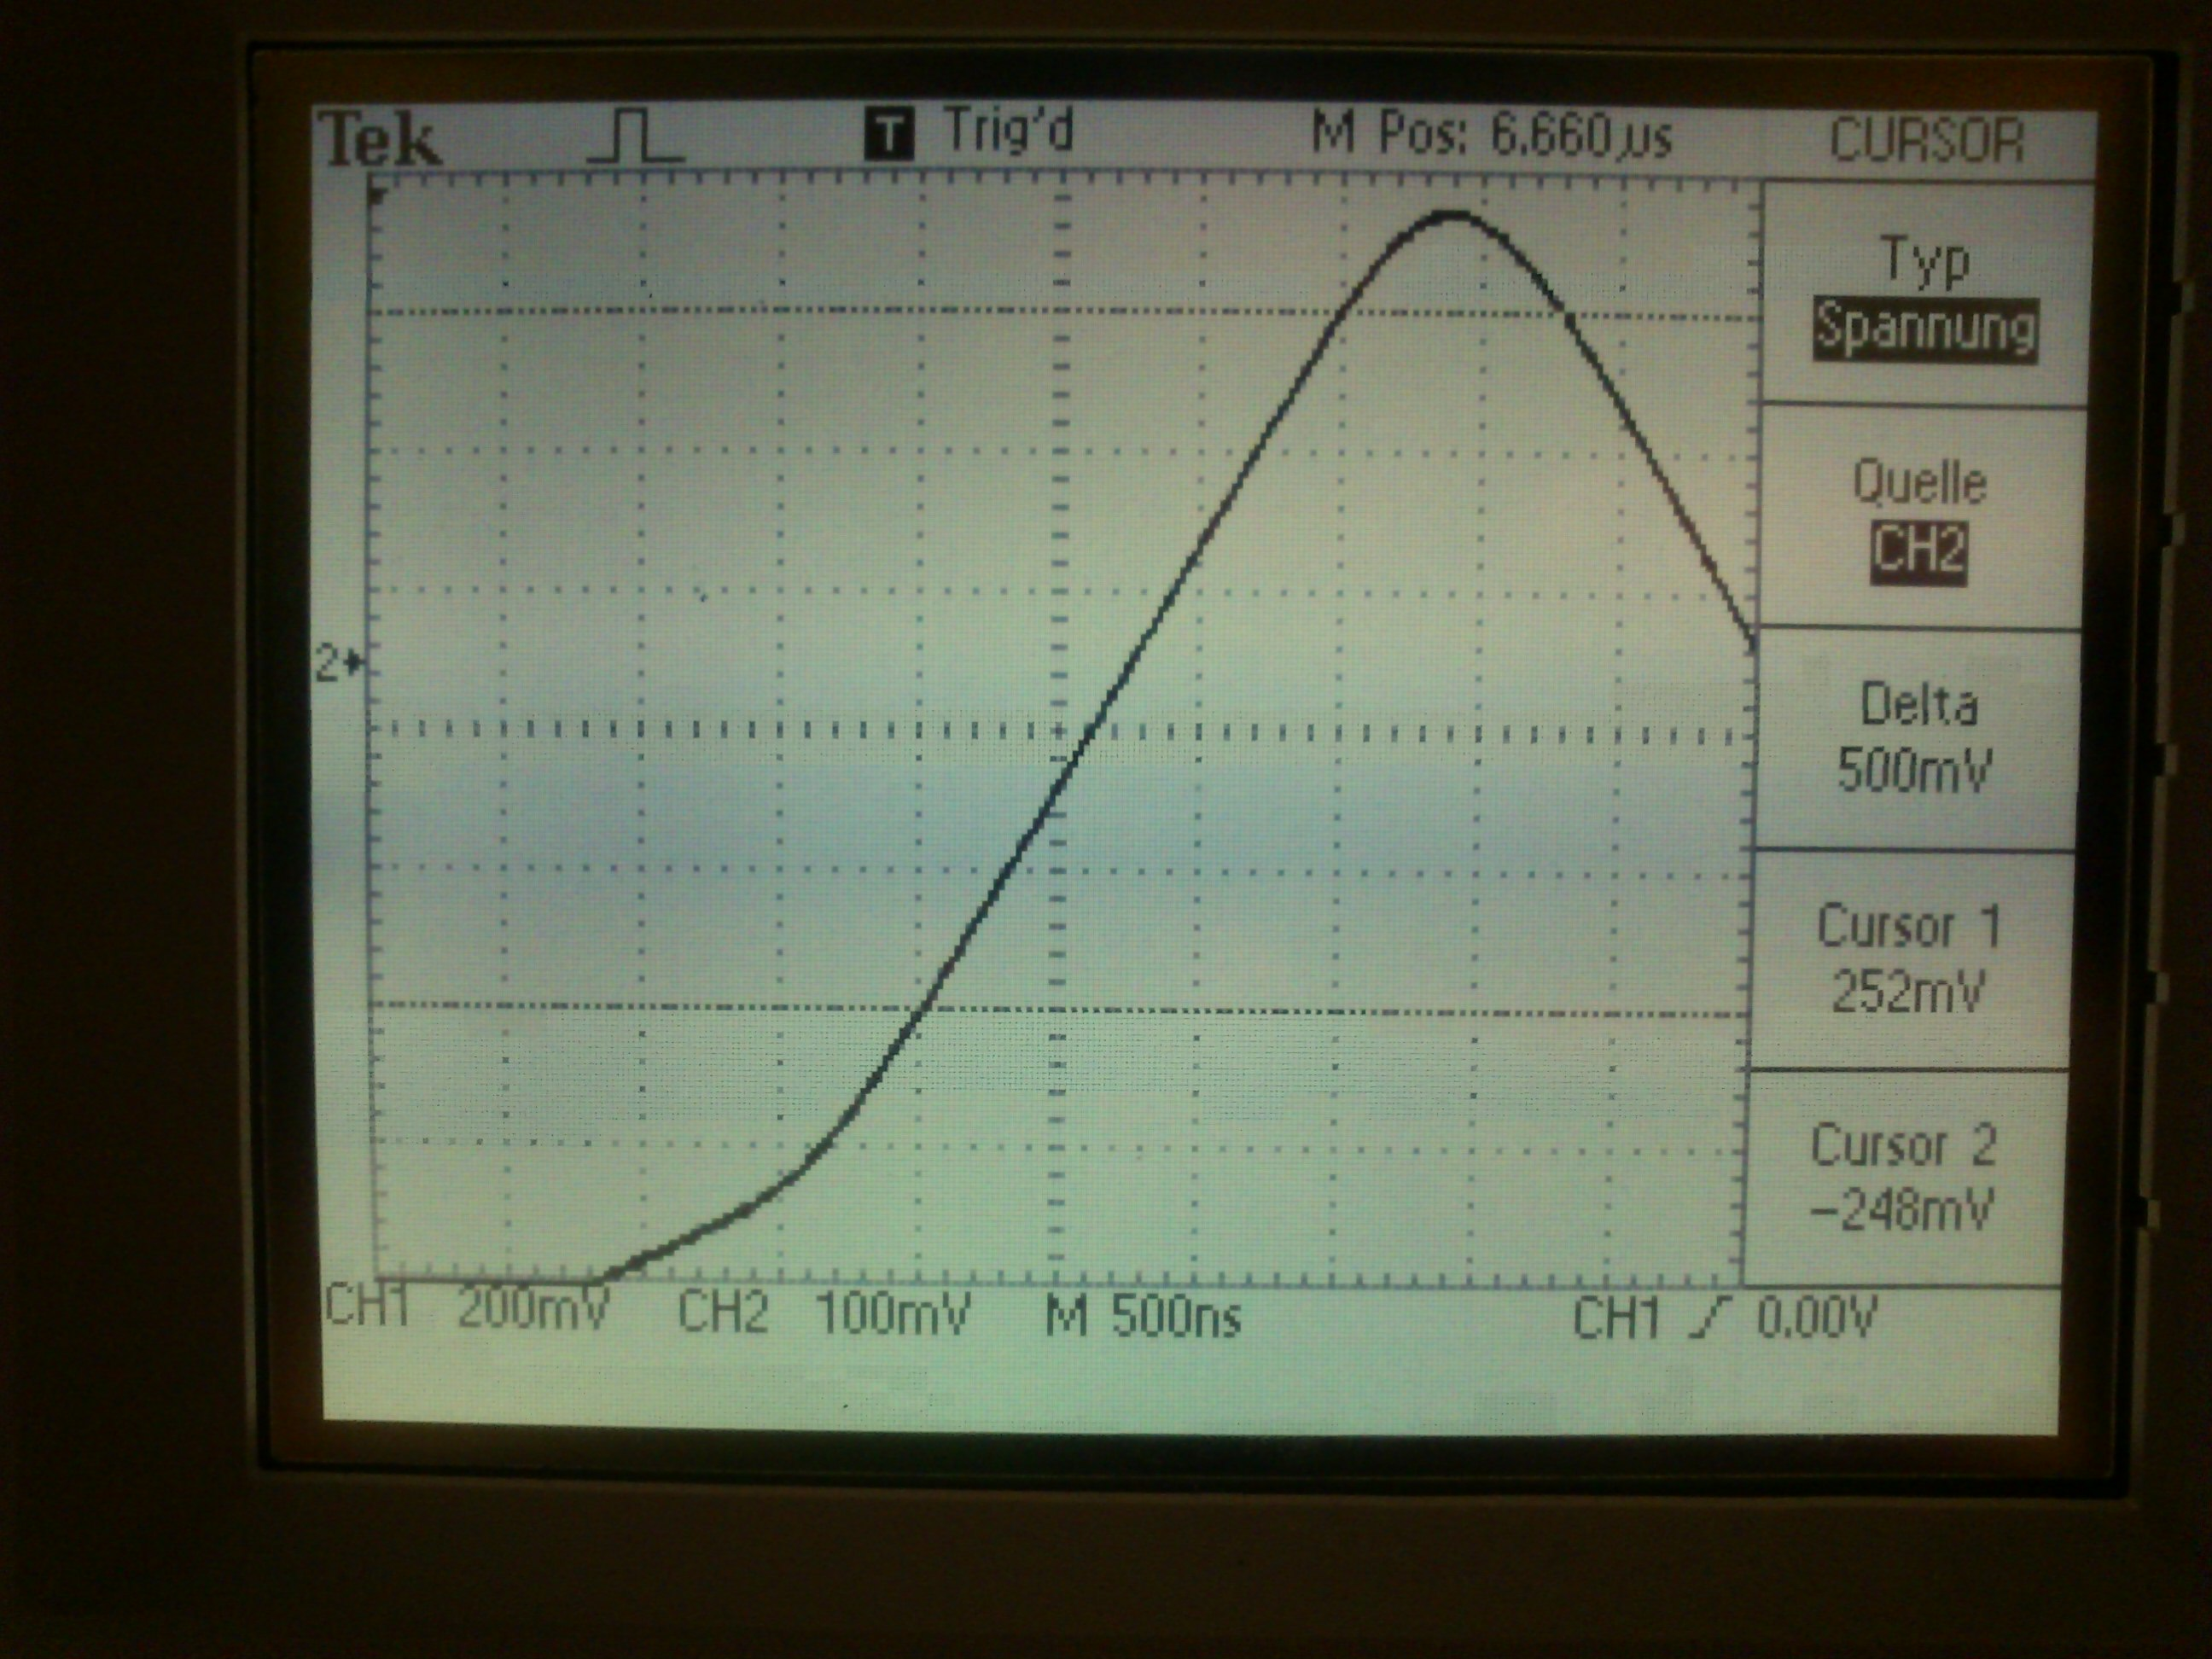
\includegraphics[width=\linewidth]{versuch6/oszi/DSC_0505.JPG}
	\caption{Bestimmung am invertierenden Verstärker}
\end{figure}

\subsection{Opamp als Komperator (Mitkopplung)}
\subsubsection*{Simulation}
\begin{figure}[H]
	\centering
	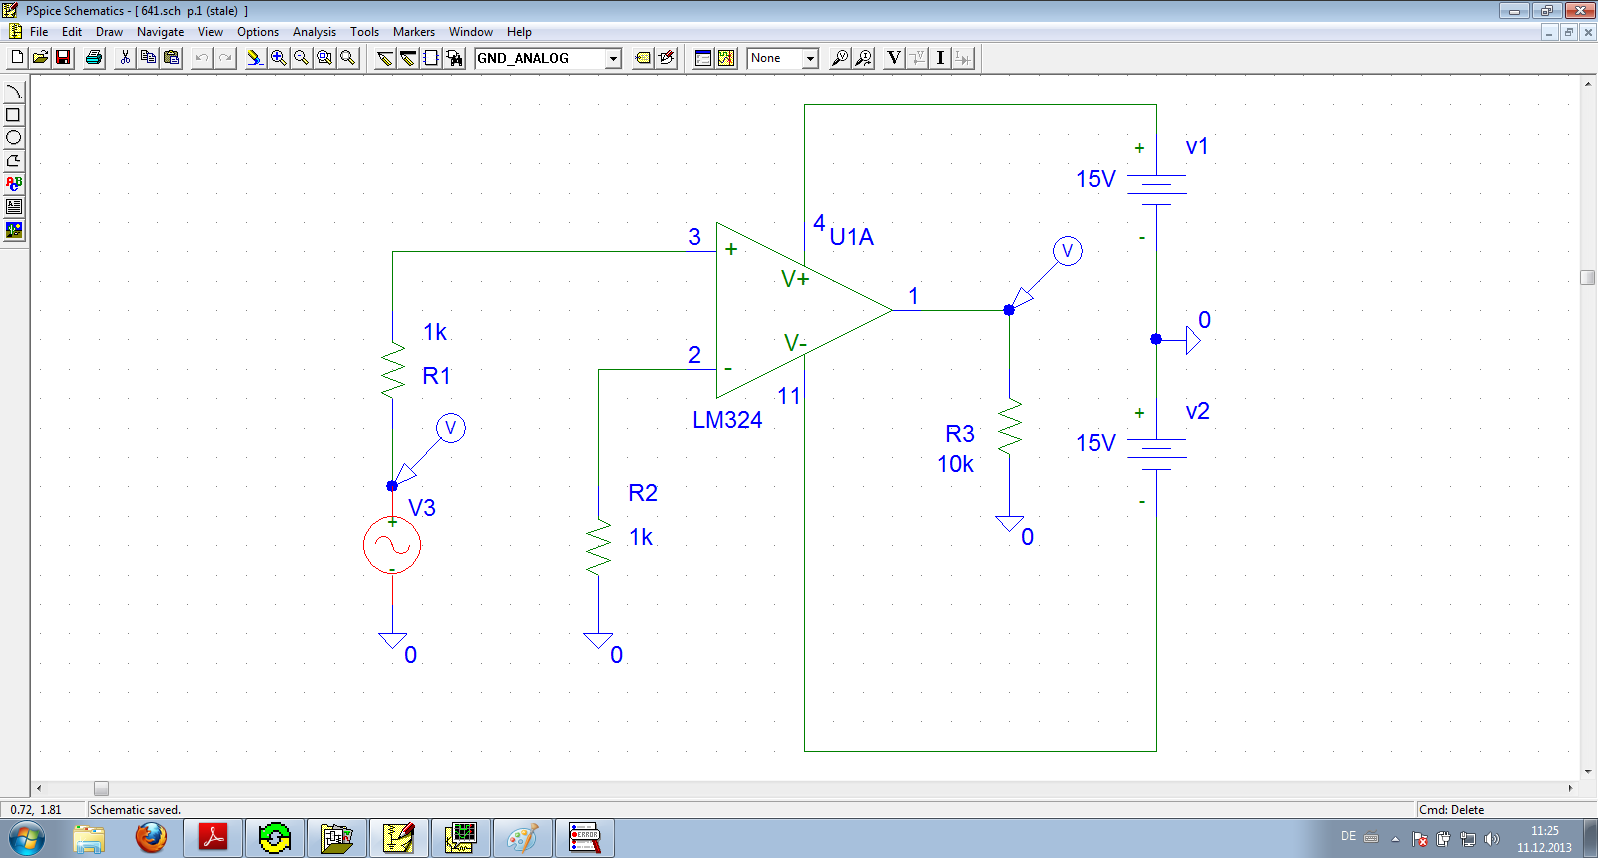
\includegraphics[width=\linewidth]{versuch6/spice/schem641.png}
	\caption{Schaltplan, wie im Skript vorgegeben}
\end{figure}
\begin{figure}[H]
	\centering
	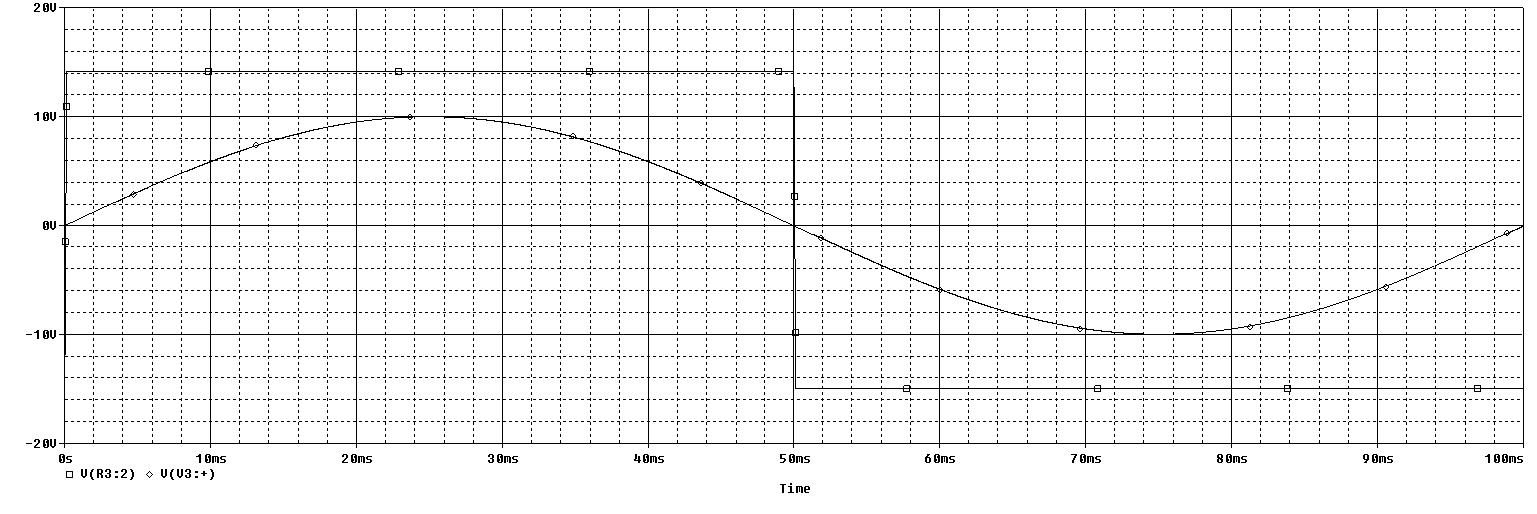
\includegraphics[width=\linewidth]{versuch6/spice/641.png}
	\caption{Simulationsergebnis}
\end{figure}
Mit Störung:
\begin{figure}[H]
	\centering
	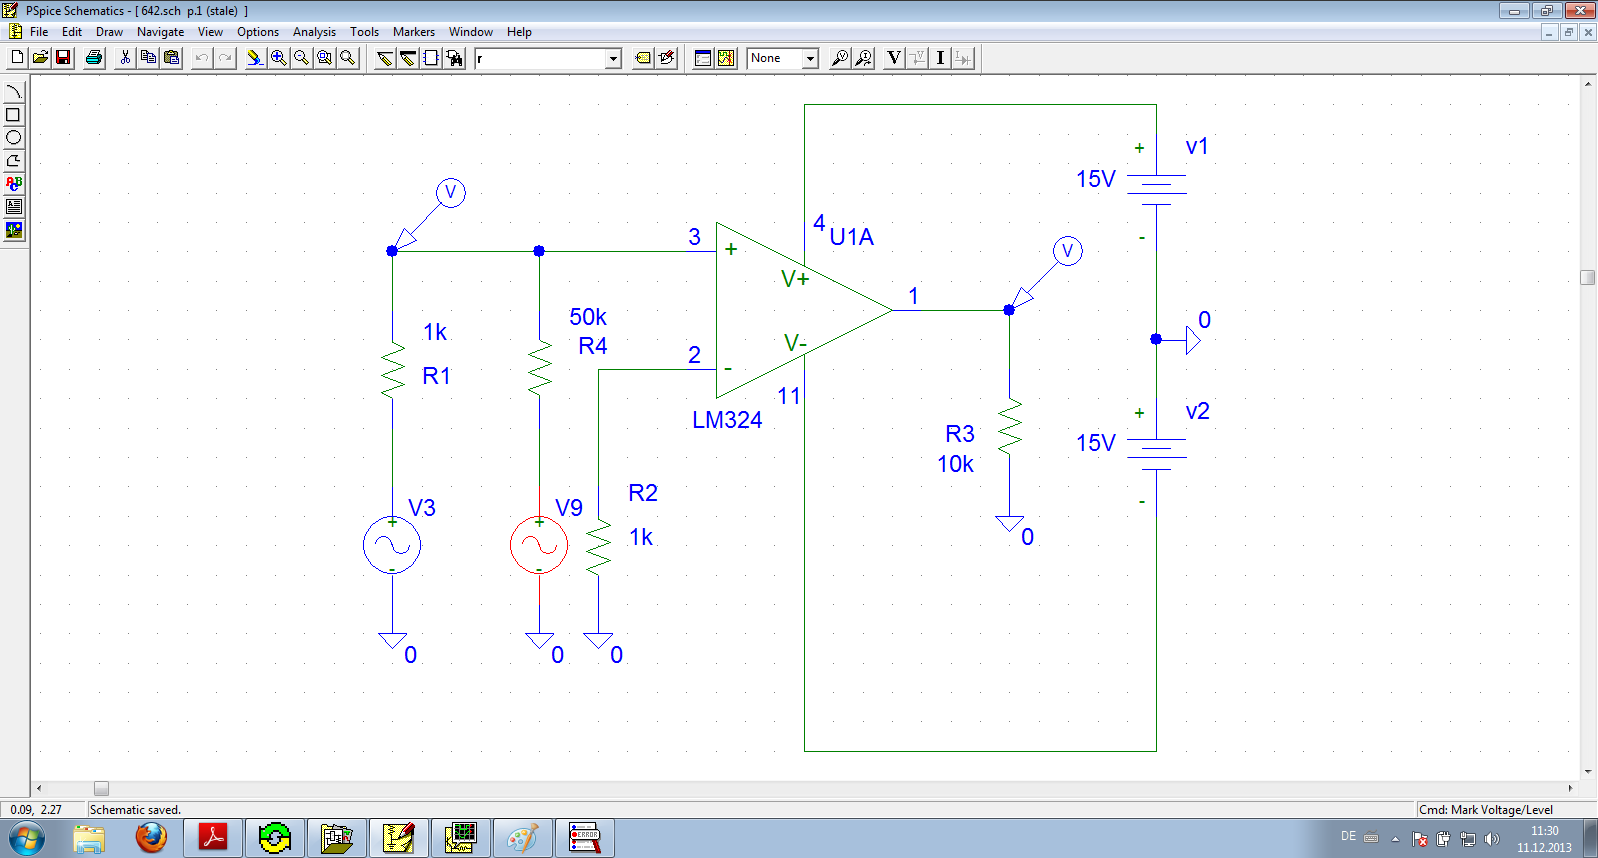
\includegraphics[width=\linewidth]{versuch6/spice/schem642.png}
	\caption{Schaltplan, wie im Skript vorgegeben}
\end{figure}
\begin{figure}[H]
	\centering
	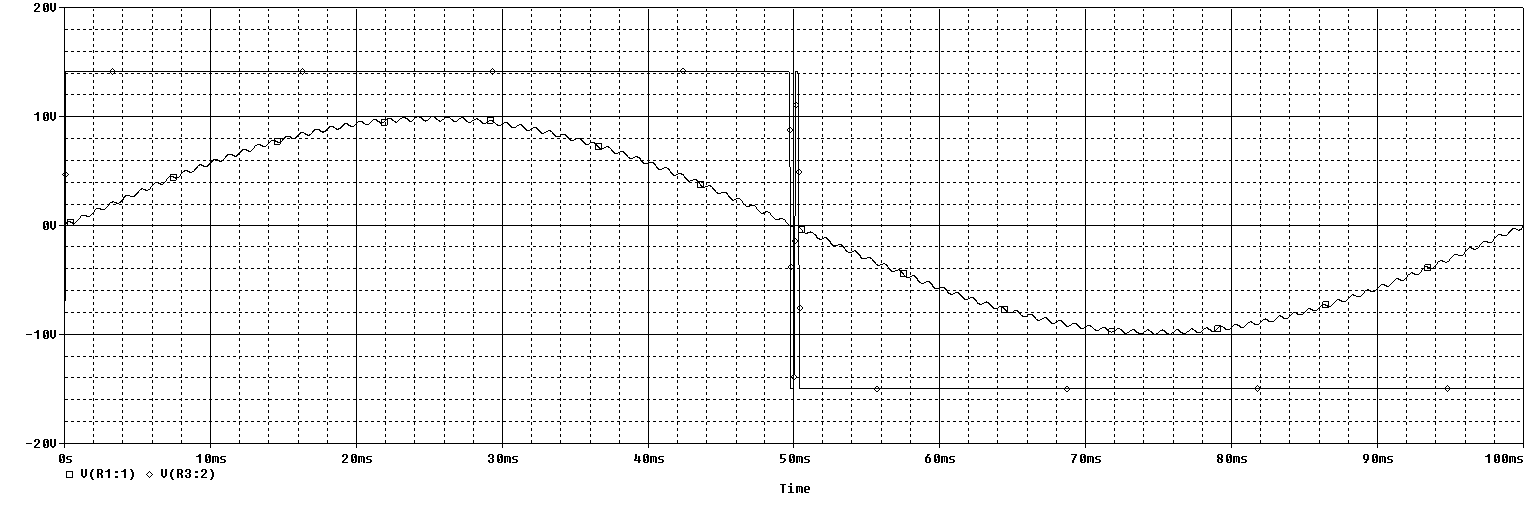
\includegraphics[width=\linewidth]{versuch6/spice/642.png}
	\caption{Simulationsergebnis}
\end{figure}
\begin{figure}[H]
	\centering
	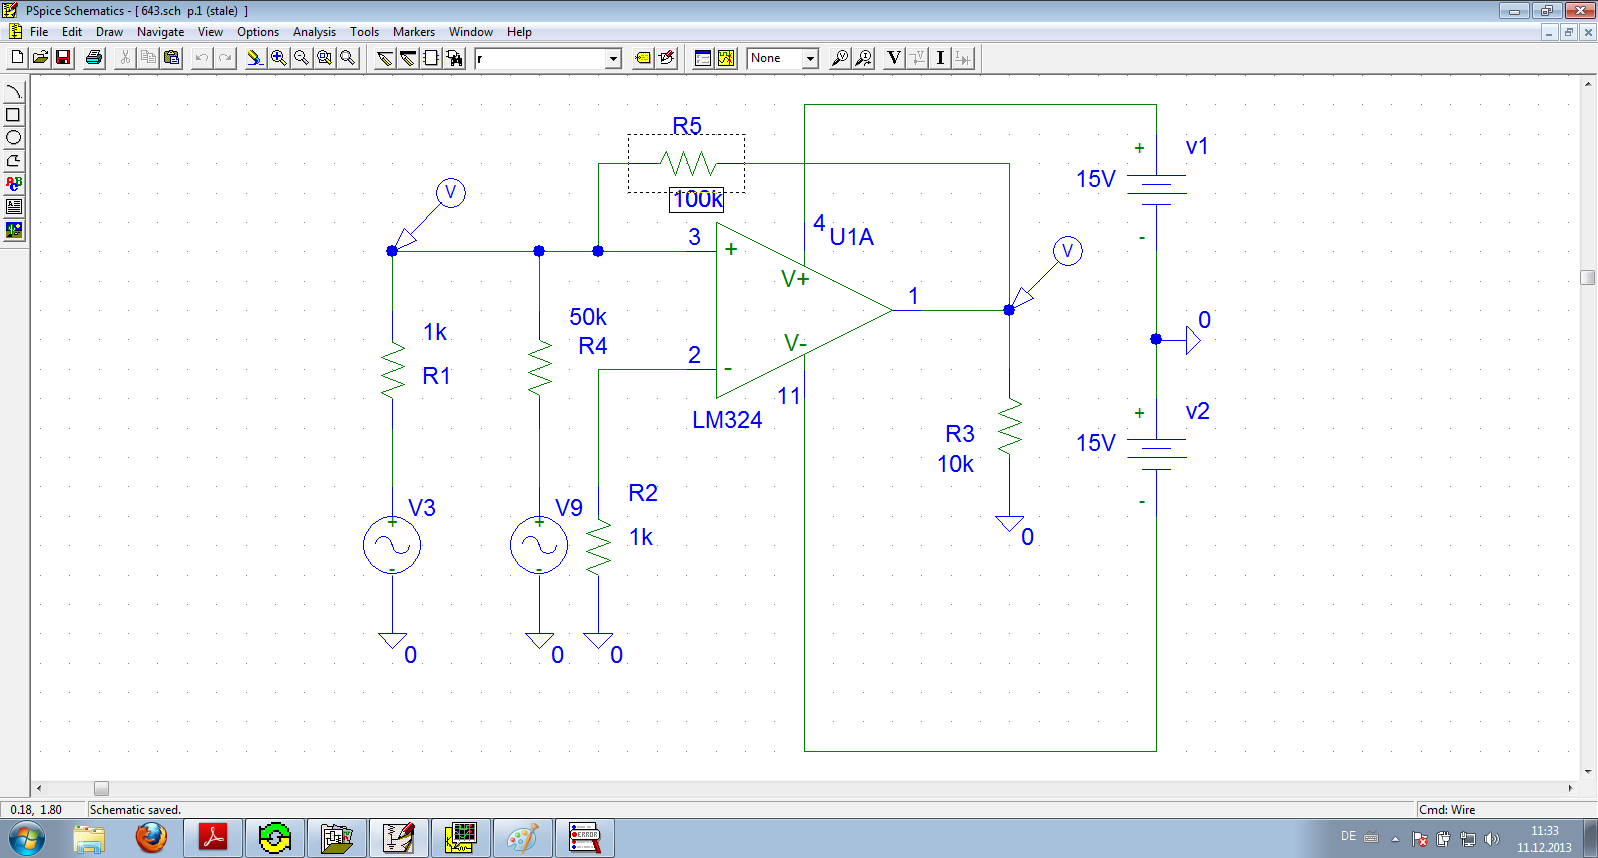
\includegraphics[width=\linewidth]{versuch6/spice/schem643.png}
	\caption{Schaltplan, wie im Skript vorgegeben}
\end{figure}
\begin{figure}[H]
	\centering
	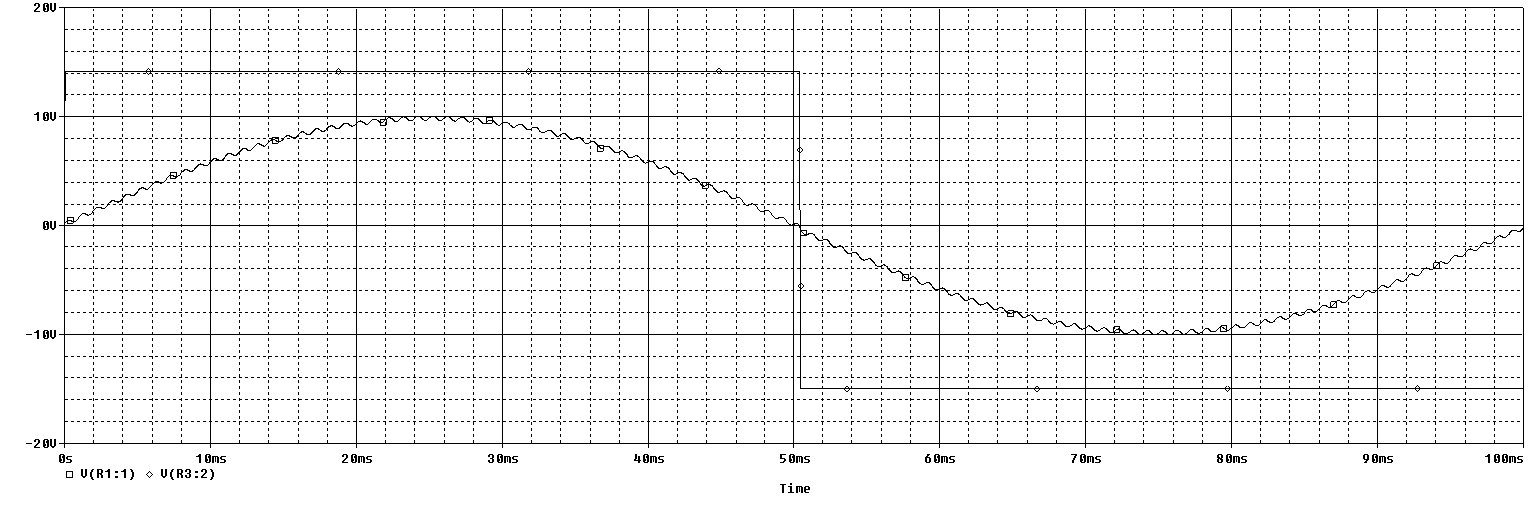
\includegraphics[width=\linewidth]{versuch6/spice/643.png}
	\caption{Simulationsergebnis}
\end{figure}
Der Widerstand $ R_5 $ zieht $ V_+ $ in Richtung des gerade anliegenden logischen Pegels und realisiert so die Mittkopplung. Wählt man $ R_5 $ klein, so erhält man den typischen Schmitt-Trigger-Effekt.%, wie man in der nächsten Simulation deutlich sehen kann.

\subsubsection*{Die reale Schaltung}
\begin{figure}[H]
	\centering
	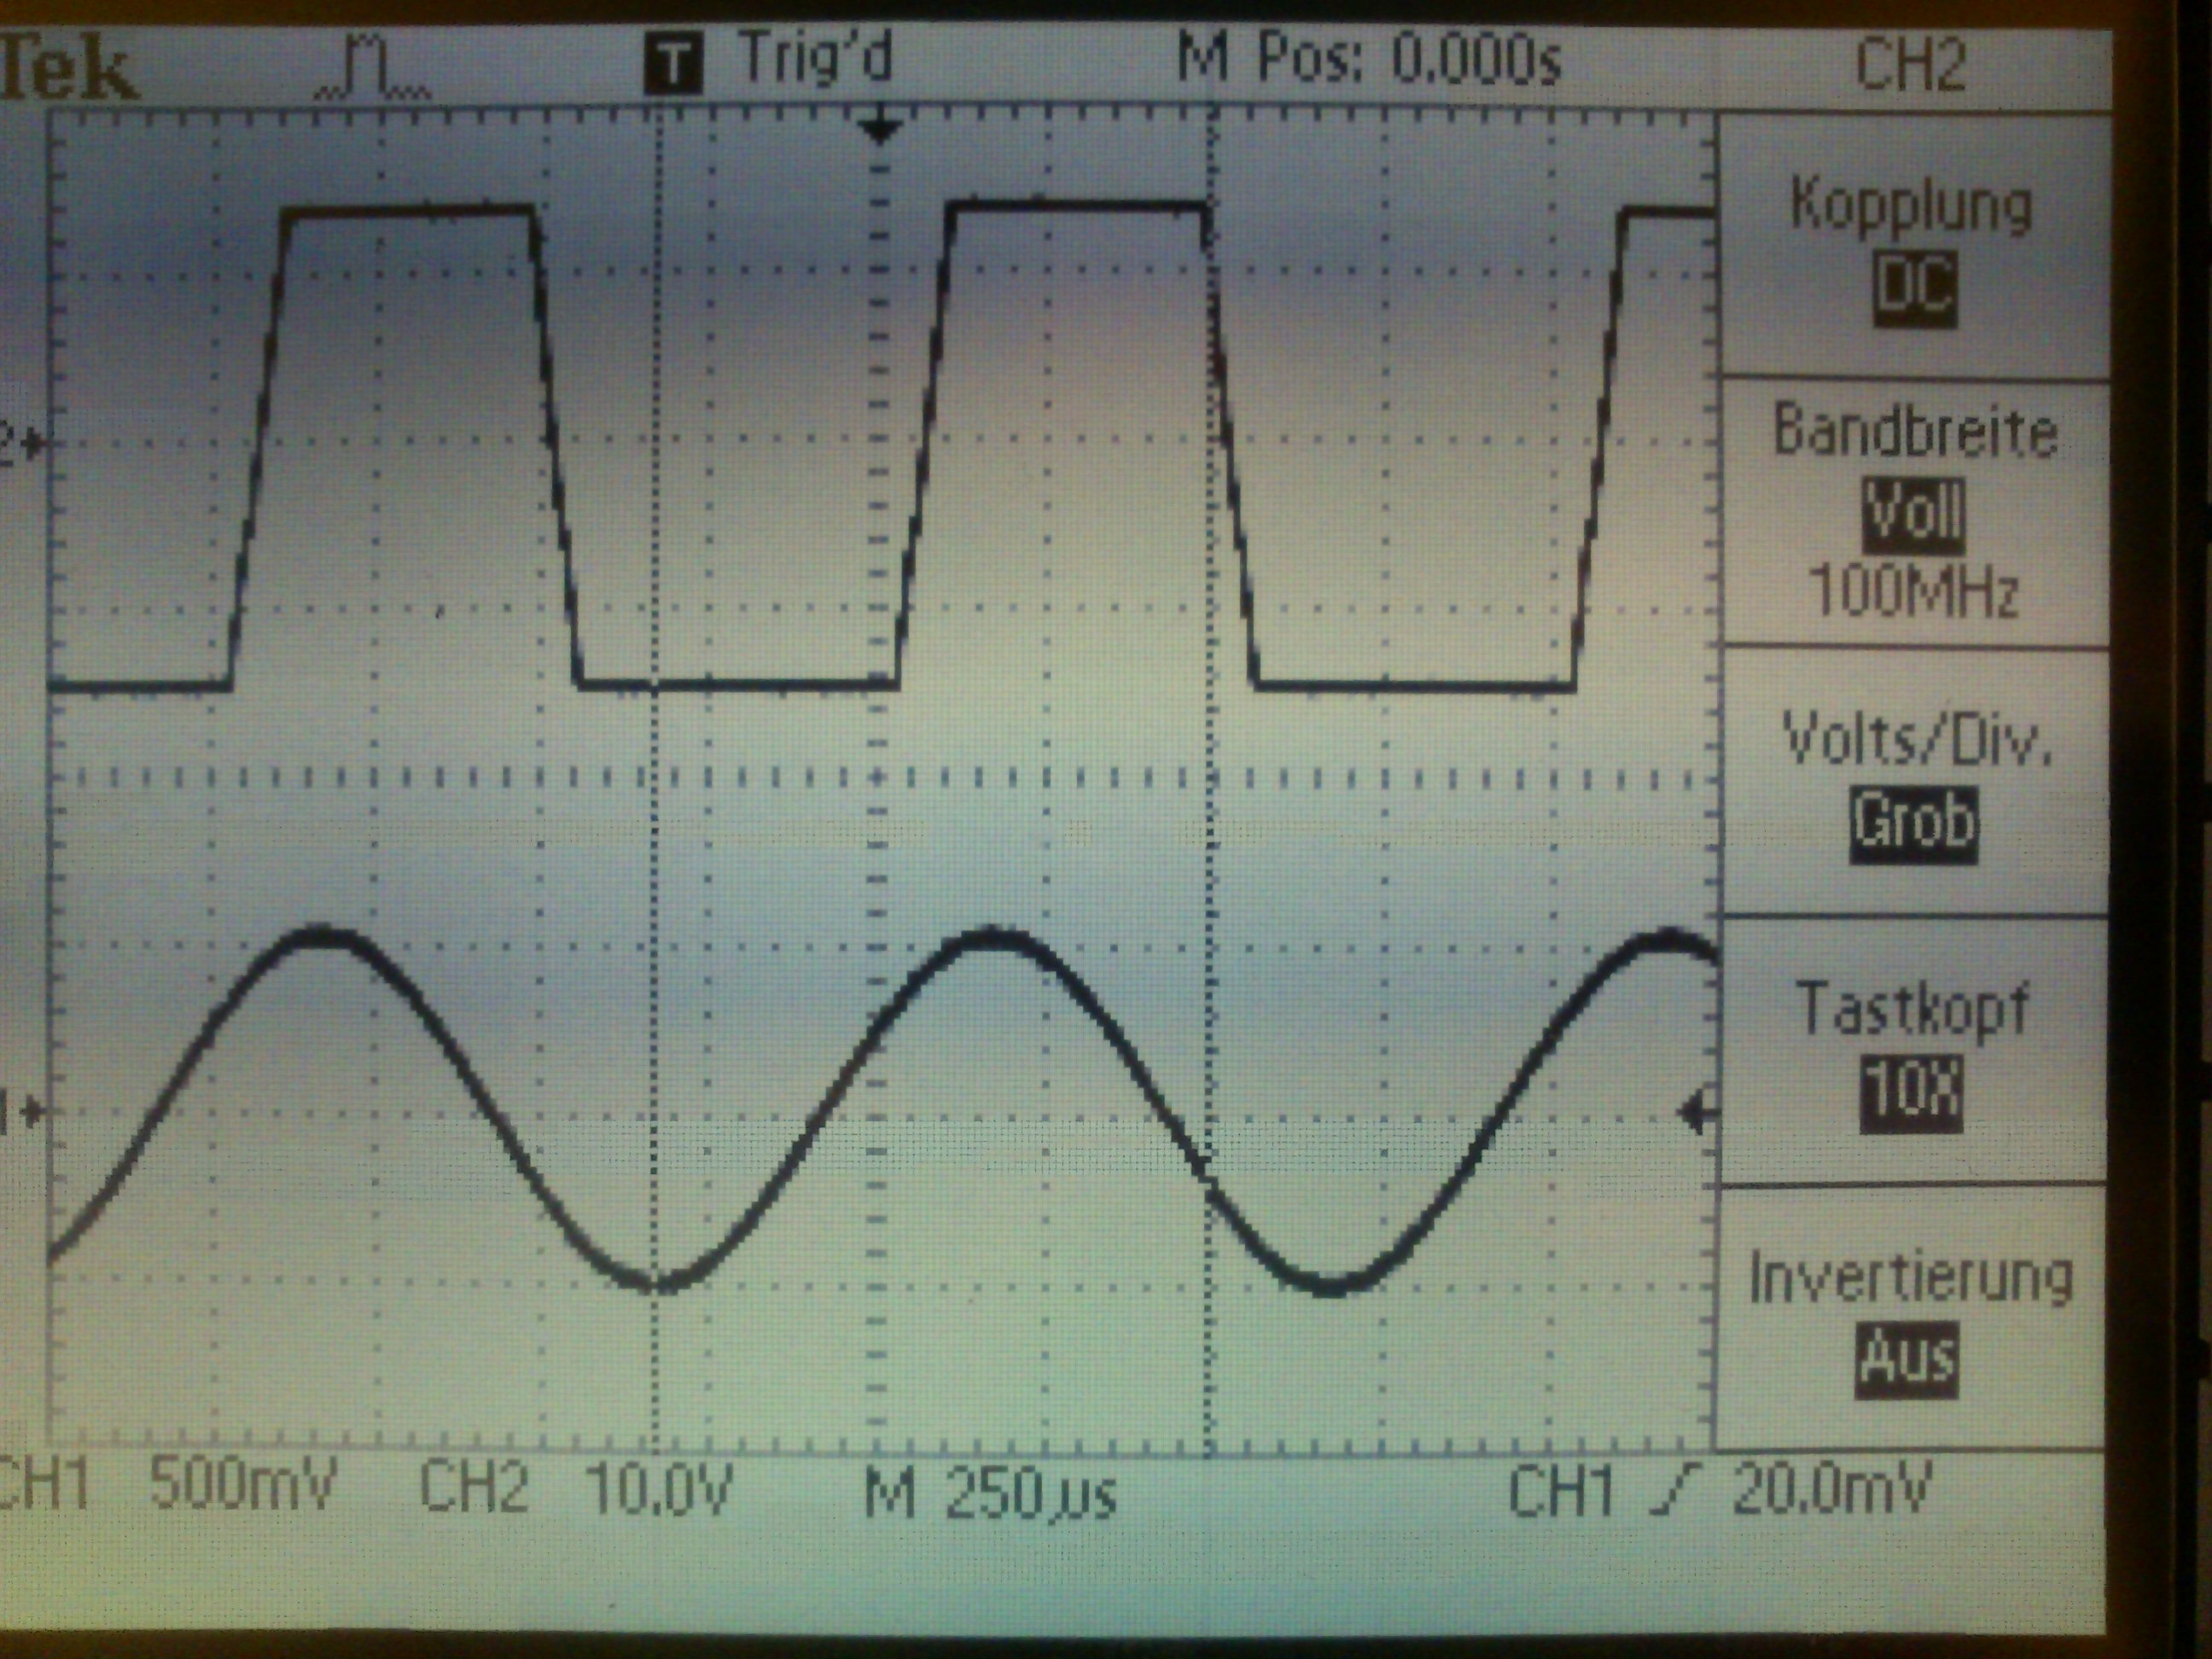
\includegraphics[width=\linewidth]{versuch6/oszi/DSC_0509.JPG}
	\caption{Die Funktion des Komperators}
\end{figure}

\subsubsection*{Schmitt-Trigger}
Dann wurde der Wert von $ R_5 $ auf 3k\Ohm verringert:
\begin{figure}[H]
	\centering
	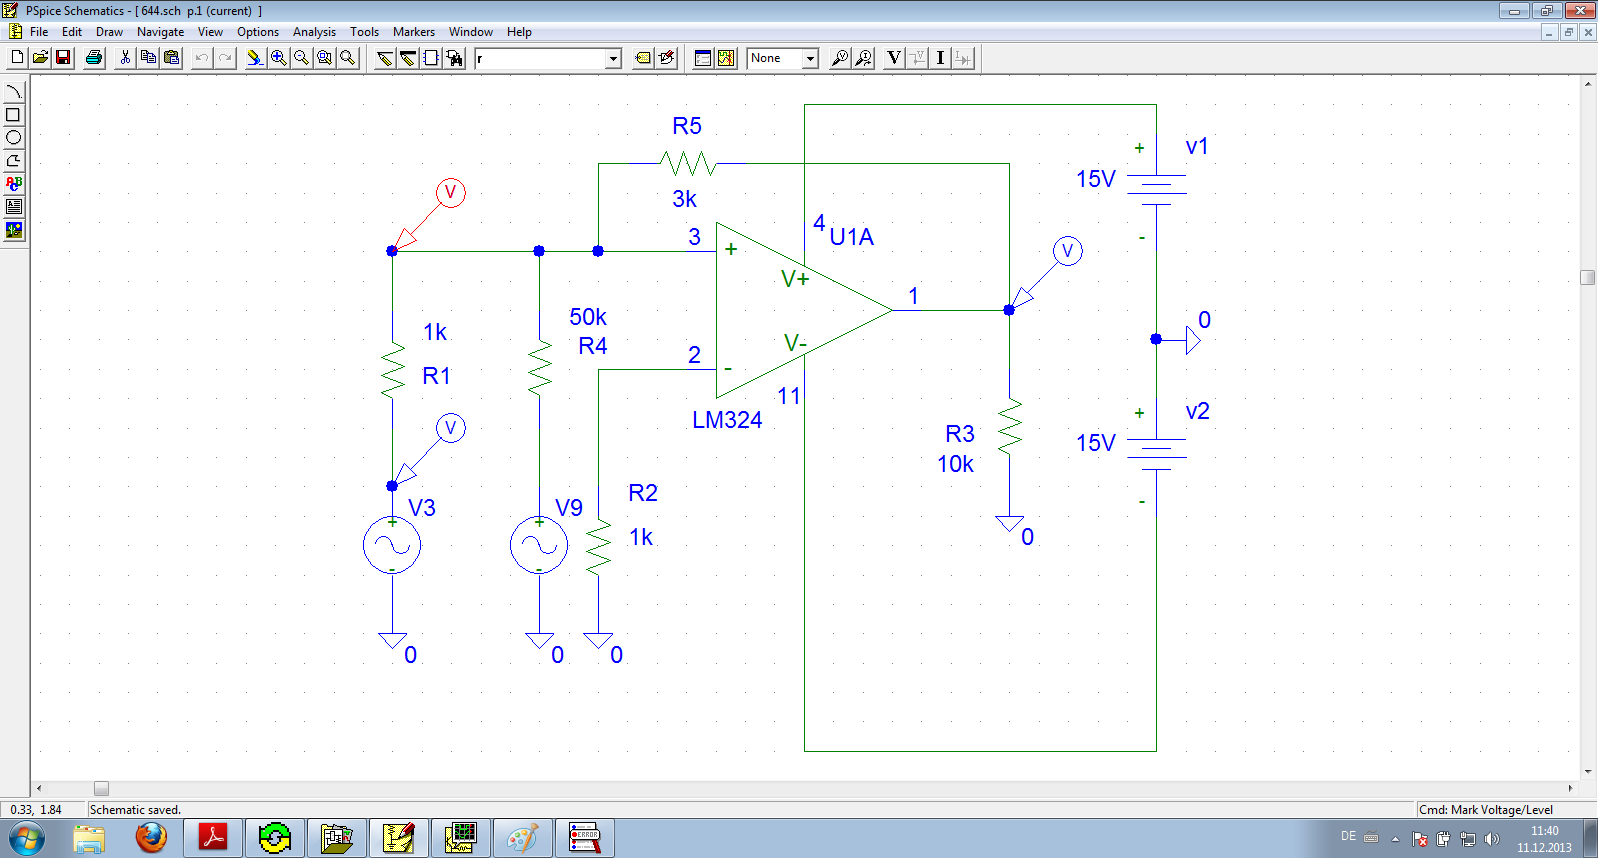
\includegraphics[width=\linewidth]{versuch6/spice/schem644.png}
	\caption{Schaltplan, wie im Skript vorgegeben}
\end{figure}
\begin{figure}[H]
	\centering
	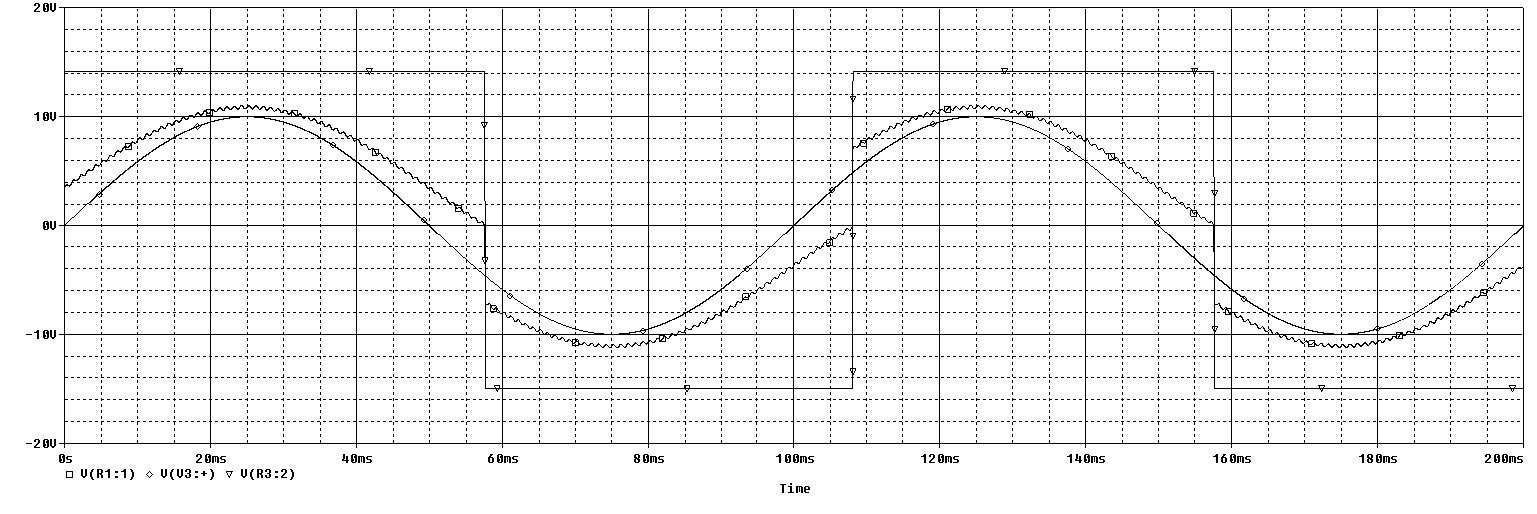
\includegraphics[width=\linewidth]{versuch6/spice/644.png}
	\caption{Simulationsergebnis: Schmitt-Trigger}
\end{figure}
Die Schaltschwelle von High nach Low wurde zu -4.5V, die von Low nach High zu 5V bestimmt. Damit ergibt sich eine Hysterese von 9.5V.\\
Ich vermute, dass mit der Frage nach dem Effekt von $ R_3 $ eigentich die Frage nach dem Effekt von $ R_5 $ gemeint war. Dessen Größe ist reziprok proportional zur Hysterese. Wenn man einen Schmitt-Trigger vor den Eingang eines Gatters setzt, so sieht dieses immer saubere Eingangssignale auch, wenn deren Störabstand eigentlich zu gering wäre.
Bei den genannten Pegeln wäre der Störabstand mit unserem Schmitt-Trigger 5V.

\subsection{Operationsverstärker als Negativimpedanzkonverter}
Die gezeigte Schaltung wird Negaivimpedanzkonverter genannt, weil sie einen negativen Widerstand emuliert.
Die Spannung am nichtinvertierenden Eingang beträgt:
\[ V_+ = \frac{-100k\Ohm}{(-100+90)k\Ohm} * V_{signalquelle} = 10 * V_{signalquelle} \]
\begin{figure}[H]
	\centering
	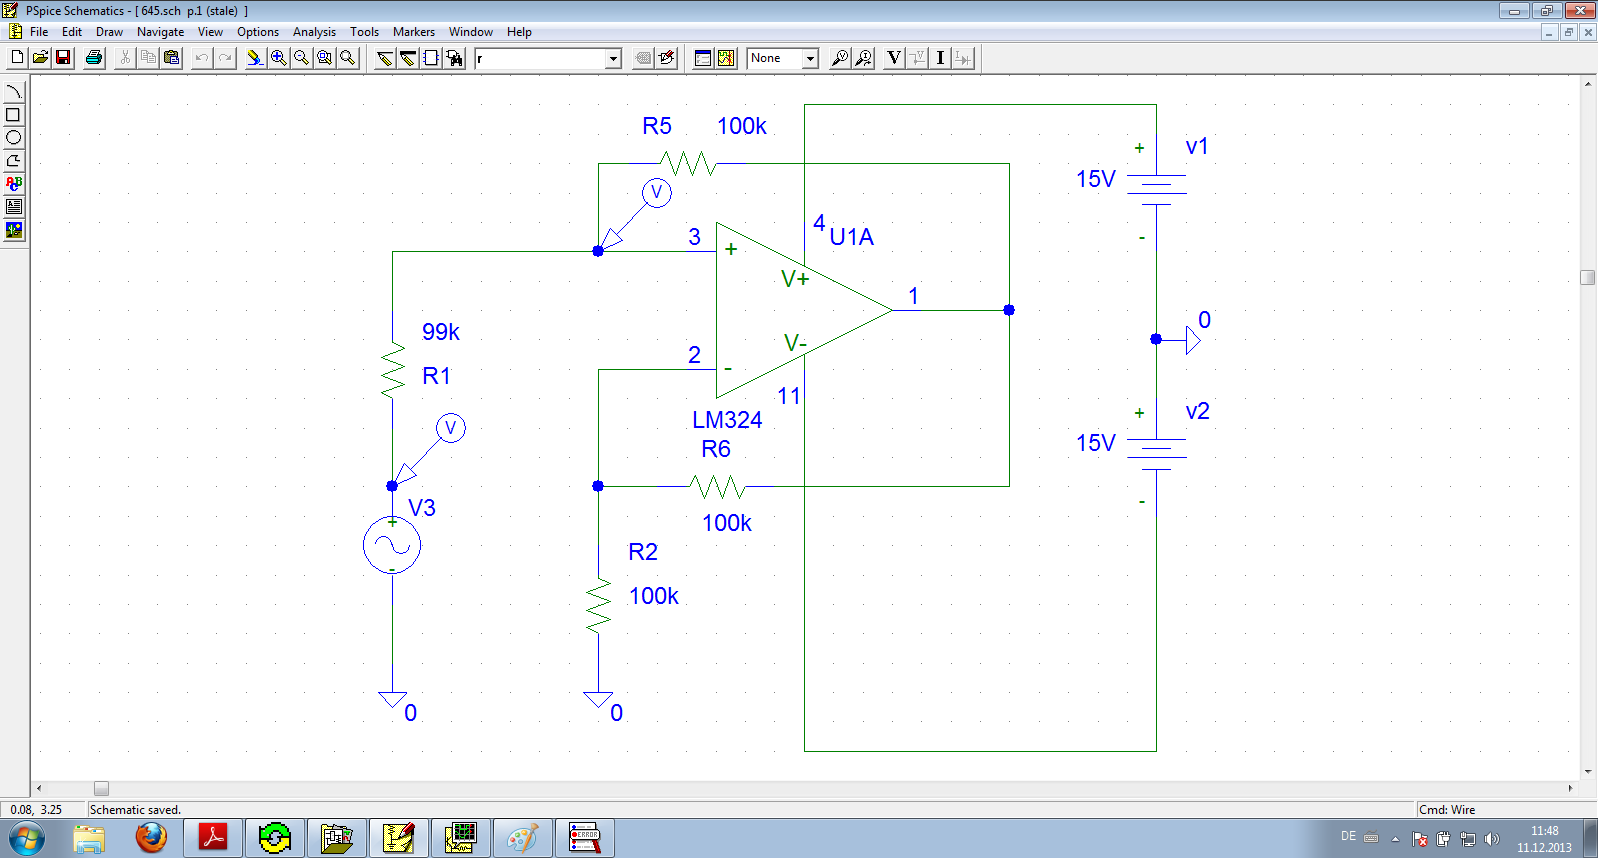
\includegraphics[width=\linewidth]{versuch6/spice/schem645.png}
	\caption{Schaltplan, wie im Skript vorgegeben}
\end{figure}
\begin{figure}[H]
	\centering
	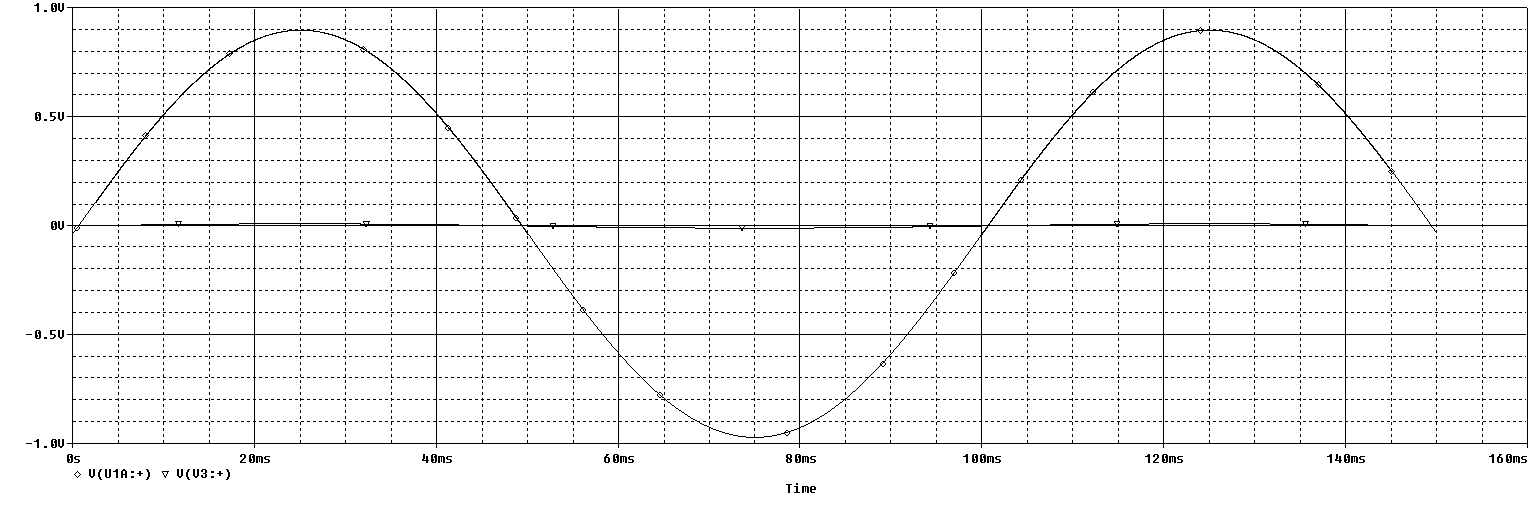
\includegraphics[width=\linewidth]{versuch6/spice/645.png}
	\caption{Simulationsergebnis}
\end{figure}
Offensichtlich ist die reale Verstärkung deutlich größer, als die berechnete.





